\chapter{The Large Hadron Collider and the \ATLAS Detector}\label{chap:lhc_atlas}

%AB: The work presented in this thesis relies on data recorded by the ATLAS detector in high energy proton-proton collisions. This chapter provides an overview of the experimental apparatus and analysis techniques used throughout this thesis.

Since the completion of its construction in 2008, the Large Hadron Collider (\LHC)~\cite{Evans:2008zzb} at \CERN has extended the frontiers of particle physics through significant increases in centre of mass energy and luminosity compared with previous collider experiments.
The \LHC accelerates bunches of protons around a \SI{27}{\km} ring until they are travelling just \SI{3}{\m\per\s} slower than than the speed of light, at which point they are made to collide.
The proton bunches travel round the ring 11,000 times per second in two concentric beams, which are guided by superconducting magnets cooled using liquid helium to \SI{-271.3}{\degreeCelsius} (\SI{1.9}{\kelvin}).
The beams travel in opposite directions around the ring and are crossed at four locations so that collisisons between protons can take place.
Around these collision points four specialised detectors, ALICE~\cite{AliceCollaboration_2008}, CMS~\cite{CMS-TDR-08-001}, LHCb~\cite{LHCbCollaboration_2008} and \ATLAS~\cite{PERF-2007-01}, are located to capture information about the products of the collisions.

In this chapter, a brief overview of the \LHC and the accelerator complex at \CERN is given in \cref{sec:lhc}.
The coordinate system used at the \ATLAS detector and other common definitions are introduced in \cref{sec:atlas_coords}.
An overview of the different detector systems is provided in \cref{sec:atlas_detector}, and finally descriptions of various commonly used reconstructed objects is given in \cref{sec:physics-objects}.


\section{The Large Hadron Collider}\label{sec:lhc}

The \LHC is operated in multi-year \textit{runs} during which beams of protons are circulated and collided.
Between runs there are periods of shutdown while the accelerator and detector machinery is maintained and upgraded.
\runone began in 2010 when the \LHC collided proton bunches, each containing more than $10^{11}$ particles, 20 million times per second, providing \SI{7}{\TeV} proton-proton collisions at instantaneous luminosities of up to \peakLumi.
The centre-of-mass energy was increased to \SI{8}{\TeV} in 2012.
Over the course of \runone, \intlumirunone of usable integrated luminosity was recorded.
\runtwo, which spanned 2015--2018, further increased the the proton-proton collision energy to \SI{13}{\TeV}.
During \runtwo the bunch spacing was reduced, leading to a collisison rate of \SI{40}{\mega\hertz}.
Over the course of \runtwo a total usable integrated luminosity of \intlumi was recorded. % less good for physics
2022 marked the beginning of \runthree which, with a higher center of mass energy and peak luminosity, is expected to culminate in an approximate tripling of the dataset size.
%We will be focusing the proton beams at the interaction points to less than 10 micron beam size, to increase the collision rate. (nominal beam size (width) is 16 microns from around run1)
A summary of key information about each run is listed in \cref{tab:lhc_runs}.

\begin{table}[!htbp]
  \footnotesize\centering
  \setlength{\tabcolsep}{0.5em} % for the horizontal padding
  \begin{tabular}{cc|cccc}
      \toprule\hline
      \textbf{Period} & \textbf{Year} & $\sqrt{s}$ [\unit\TeV] 
      & \angles{\mu} & \textbf{Bunch spacing} [\unit\ns] & \textbf{Luminosity} [\unit\invcmsqpersec] \\
      \hline
      Run 1 & 2010--2012 & \SIrange[range-phrase=--,range-units=single,range-exponents=combine]{7}{8}{} & 18 & 50--150 & $8 \times 10^{33}$ \\
      Run 2 & 2015--2018 & \SI{13  }{} & 34 & 25 & $1\textnormal{--}2 \times 10^{34}$ \\
      Run 3 & 2022--2025 & \SI{13.6}{} & 50 & 25 & $2 \times 10^{34}$ \\
      \hline\bottomrule
  \end{tabular}
  \caption{
    Overview of the different LHC runs \cite{atlas-lumi-run1,atlas-lumi-run2}.
    The average number of interactions per bunch-crossing is denoted as \angles{\mu} (see \cref{sec:collider_defs}), and is here averaged over the entire run.
    The luminosity is the peak instantaneous luminosity. 
    Numbers for Run 3 are preliminary and are only provided to give an indication of expected performance.
    % run 1 run 2 trigger https://cds.cern.ch/record/2058218/
    %  2-3 × 1034 cm−2 s−1 and an average pile-up of ~80 collisions/bunch-crossing
    % https://cds.cern.ch/record/2732959/files/LHCP2020_094.pdf
  }
  \label{tab:lhc_runs}
\end{table}

An overview of the accelerator complex at CERN is shown in \cref{fig:accelerator_complex}.
The LHC is at the final stage of a chain of accelerators which incrementally step-up the energy of incoming protons.
The first accelerator is Linac2 (which has been replaced by Linac4 in 2020), a linear accelerator which accelerates negative hydrogen ions to an energy of \SI{160}{\MeV}.
Upon leaving Linac4, the ions are stripped of both electrons and the resulting protons are fed into the Proton Synchrotron Booster (PSB), which increases the energy of the protons to \SI{2}{\GeV}.
The protons leaving the PSB are passed to the Proton Synchrotron (PS), which increases the energy to \SI{26}{\GeV}, and then from the PS to the Super Proton Synchrotron (SPS) which further increases the energy to \SI{450}{\GeV}.
Finally, the proton beams are injected in the LHC where they are accelerated to their final energy of \SI{6.5}{\TeV} (for \runtwo).

\begin{figure}[!htbp]
  \centering
  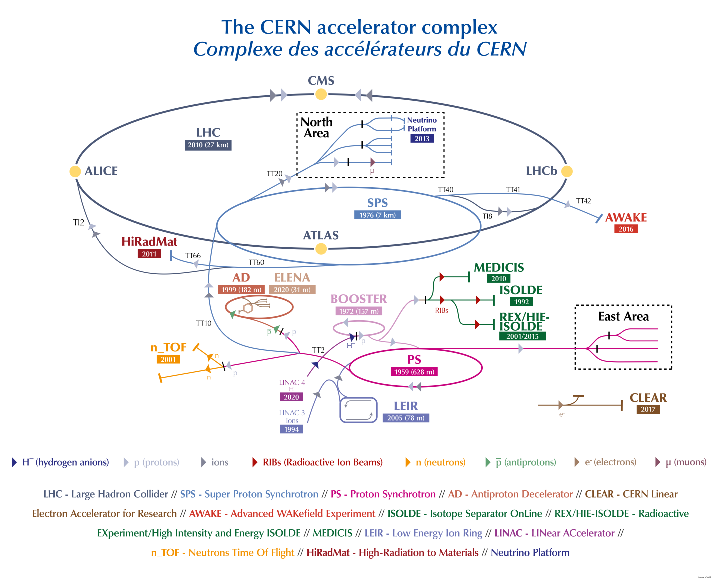
\includegraphics[width=\textwidth]{chapters/2.detector/figs/accelerator_complex.pdf}
  \caption{
    An overview of the \CERN accelerator complex \cite{CERN:2012:accelerators}.
    The \LHC is fed by a series of accelerators starting with Linac2 (or Linac4 from 2020).
    Next are the Proton Synchrotron Booster, the Proton Synchrotron, and finally the Super Proton Synchrotron which injects protons into the \LHC.
  }
  \label{fig:accelerator_complex}
\end{figure}


\section{Coordinate System \& Collider Definitions}\label{sec:atlas_coords}

In \cref{sec:coord_sys}, the coordinate system used at \ATLAS is introduced.
The parameterisation used for specifying the trajectory of charged particle tracks is described in \cref{sec:track_parameterisation}, and definitions for some frequently occurring concepts and quantities is provided in \cref{sec:collider_defs}.

\subsection{ATLAS Coordinate System}\label{sec:coord_sys}

%% based on https://twiki.cern.ch/twiki/bin/view/AtlasProtected/PubComCommonText

The origin of the coordinate system used by \ATLAS is the nominal interaction point in the centre of the detector.
As shown in \cref{fig:atlas_coord_system}, the \axis{z} points along the direction of the beam pipe, while the \axis{x} points from the interaction point to the centre of the LHC ring, and the \axis{y} points upwards.
The transverse plane lies in $x$\nobreakdash-$y$ while the longitudinal plane lies along the \axis{z}.
A cylindrical coordinate system with coordinates $(r,\phi)$ is used in the transverse plane, where $r$ is the radius from the origin and $\phi$ is the azimuthal angle around the \axis{z}.

\begin{figure}[!htbp]
  \centering
  % Author: Izaak Neutelings (June 2017)
% taken from https://tex.stackexchange.com/questions/159445/draw-in-cylindrical-and-spherical-coordinates
% Licensed under CC Attribution-Share Alike 4.0 International  https://creativecommons.org/licenses/by-sa/4.0/
% Original source https://wiki.physik.uzh.ch/cms/latex:example_spherical_coordinates
% Modifications by Giles Strong (March 2020):
% 1. Removal of some header code
% 2. Changing theta to eta
% 3. Addition of mountains
% 4. Changed "\draw[dashed,red] (O)  -- (Pxy);" to "\draw[->] (O)  -- (Pxy) node[right] {$p_t$};"
% Modifications by Giles Strong (April 2020):
% 1. Removal of Jura mountains
% 2. Rotated to be in terms of ATLAS coordinate system
% 3. Resized labels for the detectors

\tikzset{>=latex} % for LaTeX arrow head

\tdplotsetmaincoords{75}{50} % to reset previous setting 75 50
    \begin{tikzpicture}[scale=2.7,tdplot_main_coords,rotate around x=90]
    
    % variables
    \def\rvec{1.2}
    \def\thetavec{40}
    \def\phivec{70}
    \def\R{1.1}
    \def\w{0.3}
    
    % axes
    \coordinate (O) at (0,0,0);
    \draw[thick,->] (0,0,0) -- (1,0,0) node[below left]{$x$};
    \draw[thick,->] (0,0,0) -- (0,1,0) node[below right]{$y$};
    \draw[thick,->] (0,0,0) -- (0,0,1) node[below right]{$z$};
    \tdplotsetcoord{P}{\rvec}{\thetavec}{\phivec}
    
    % vectors
    \draw[->,red] (O) -- (P) node[above left] {$\overrightarrow{p}$};
    \draw[->] (O)  -- (Pxy) node[right] {$p_t$};
    \draw[dashed,red] (P)  -- (Pxy);
    \draw[dashed,red] (Py) -- (Pxy);
    
    % circle - LHC
    \tdplotdrawarc[thick,rotate around x=90,black!70!blue]{(\R,0,0)}{\R}{0}{360}{}{}
    
    % compass - the line between CMS and ATLAS has a ~12° declination (http://googlecompass.com)
    \begin{scope}[shift={(1.1*\R,0,1.65*\R)},rotate around y=12]
        \draw[<->,black!50] (-\w,0,0) -- (\w,0,0);
        \draw[<->,black!50] (0,0,-\w) -- (0,0,\w);
        \node[below right,black!50,scale=0.6] at (\w,0,0) {N};
    \end{scope}
    
    % nodes
    \node[right] at (\R,0,0) {LHC};
    \fill[radius=0.8pt,black!20!red]
        (O) circle node[left=4pt,below=5pt] {ATLAS};
    \draw[thick] (0.02,0,0) -- (0.5,0,0); % partially overdraw x-axis and CMS point
    \fill[radius=0.8pt,black!20!blue]
        (2*\R,0,0) circle
        node[right=4pt,below=2pt,scale=0.7] {CMS};
    \fill[radius=0.8pt,black!10!orange]
        ({-\R*sqrt(2)/2+\R},0,{-\R*sqrt(2)/2}) circle % 45 degrees from ATLAS
        node[left=2pt,below=2pt,scale=0.7] {ALICE};
    \fill[radius=0.8pt,black!60!green]
        ({-\R*sqrt(2)/2+\R},0,{\R*sqrt(2)/2}) circle % 45 degrees from ATLAS
        node[below=6pt,right=3pt,scale=0.7,anchor=north east] {LHCb};
    
    % arcs
    \tdplotdrawarc[->]{(O)}{0.2}{0}{\phivec}
        {above=2pt,right=-1pt,anchor=mid west}{$\phi$}
    \tdplotdrawarc[->,rotate around z=\phivec-90,rotate around y=-90]{(0,0,0)}{0.5}{0}{\thetavec}
        {anchor=mid east}{$\eta$}
\end{tikzpicture}
  \caption{
    The coordinate system used at the \ATLAS detector, showing the locations of the four main experiments located at various points around the LHC.
    The 3-vector momentum $\bm{p} = (p_x, p_y, p_z)$ is shown by the red arrow.
    Reproduced from \rcite{Strong:2020mge}.
  }
  \label{fig:atlas_coord_system}
\end{figure}


%The pseudorapidity is defined in terms of the polar angle $\theta$ as $\eta = -\ln \tan(\theta/2)$.

The polar angle $\theta$ is commonly specified in terms of the pseudorapidity $\eta$, defined as
%
\begin{equation}\label{eq:pseudorap}
  \eta = - \ln \left[ \tan \left( \frac{\theta}{2} \right) \right] .
\end{equation}
%
The pseudorapidity is a convenient quantity to work with as differences in $\eta$ are invariant under Lorentz boosts.
%In addition, particle production is constant as a function of $\eta$.

The transverse momentum \pt of an object is the sum in quadrature of the momenta in the transverse plane
%
\begin{equation}\label{eq:pt}
  \pt = \sqrt{ {p_x}^2 + {p_y}^2 } .
\end{equation}

Angular distance between two objects is measured in units of $\DeltaR$ and is defined as
%
\begin{equation}\label{eq:delta_r}
  \DeltaR = \sqrt{(\Delta\eta)^{2} + (\Delta\phi)^{2}} ,
\end{equation}
%
where $\Delta \eta$ and $\Delta \phi$ are the differences in pseudorapidity and azimuthal angle between the two objects.


\subsection{Track Parameterisation}\label{sec:track_parameterisation}

The trajectories of charged particle tracks are parameterised as a helix which is fully specified using five parameters: $(\dzero, \zzero, \phi, \theta, q/p)$.
The transverse and longitudinal impact pararameters (IP) \dzero and \zzero specify the closest approach of the trajectory of a particle to an given origin, where the hard scatter primary vertex (see \cref{sec:vertex_reco}) is used in this thesis.
$\phi$ and $\theta$ are the azimuthal and polar angles respectively, and $q/p$ is the measured charge on the track\footnote{Reconstructed charged particles are assumed to have a charge of $\pm 1$.} divided by the scalar 3-momentum.
\cref{fig:track_params} shows each of these parameters diagrammatically.

\begin{figure}[!htbp]
  \centering
  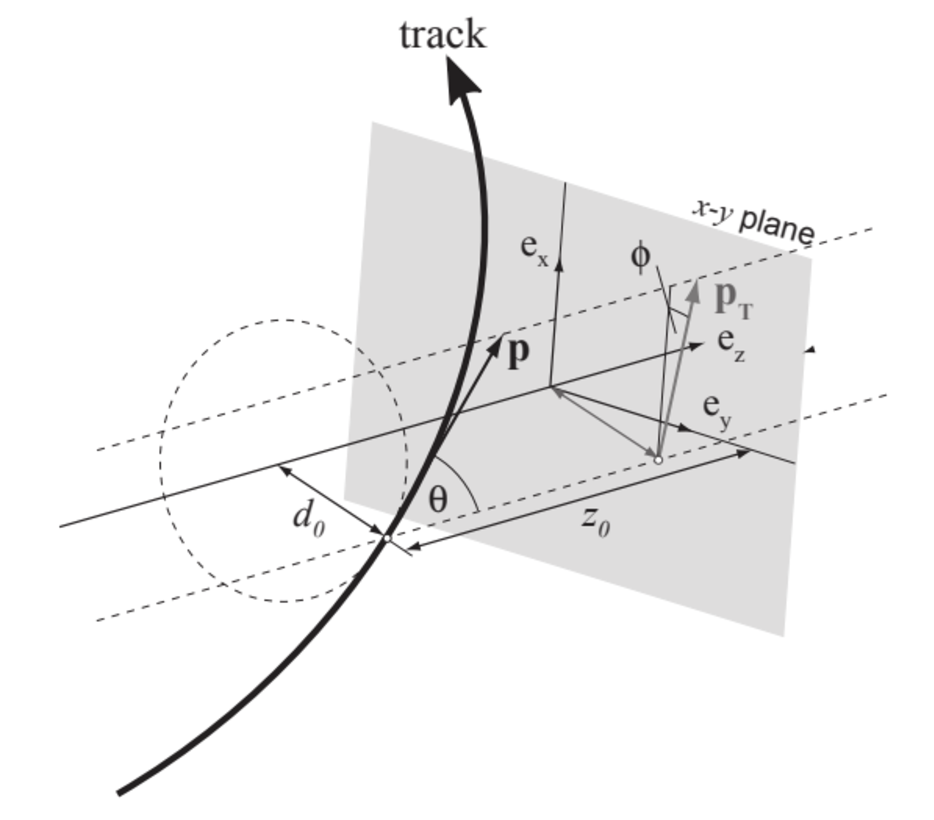
\includegraphics[width=0.75\textwidth]{chapters/2.detector/figs/track_params.pdf}
  \caption{
    The track parameterisation used at the \ATLAS detector.
    Five coordinates $(\dzero, \zzero, \phi, \theta, q/p)$ are specified, defined at the track's point of closest approach to the nominal interaction point at the origin of the coordinate system.
    The figure shows the three-momentum $\mathbf{p}$ and the transverse momentum \pt (defined in \cref{eq:pt}).
    The basis vectors $e_{\mathrm{x}}$, $e_{\mathrm{y}}$ and $e_{\mathrm{z}}$ are also shown.
    Reproduced from \rcite{atlastrackingdocs}.
  }
  \label{fig:track_params}
\end{figure}

Impact parameter significances are defined as the IP divided by its corresponding uncertainty, $\dzerosig = d_0 / \dzerouncert$ and $\zzerosig = z_0 / \zzerouncert$.
When used in flavour tagging (see \cref{chap:tracking}), track IP significances are lifetime signed according to the track's direction with respect to the jet axis and the primary vertex \cite{PERF-2012-04}.
The signed IP significances is positive if the track crosses the jet axis in front of the primary vertex and negative if the crossing is behind the primary vertex.

%\textbf{Lorentz angle}. The Lorentz angle $\theta_L$ is the angle between the electric field and the direction of the drift of the electron and holes in a silicon strip or pixel detector, when submerged in a magnetic field.

\subsection{Hadron Collider Definitions}\label{sec:collider_defs}

\subsubsection{Cross Section}
The cross section $\sigma$ is closely related to the probability of an interaction between two colliding particles, and is analogous to an effective cross-sectional area of the particles.
The cross section of a process depends on the transition matrix element and a phase space integral.
At hadron colliders such as the \LHC, the proton-proton cross section can be factorised as 
%
\begin{equation}
  \sigma(pp \to X) \approx \textnormal{PDFs} \cdot \textnormal{partonic cross section} .
\end{equation}
%
The partonic cross section can be calculated at high energies such as those found at the LHC, while the parton distribution functions (PDFs) have to be extracted from experimental results. 

\subsubsection{Luminosity}
The total number of proton-proton collisisons $N$ is related to the total $pp$ cross $\sigma$ section by the integrated luminosity $L$, as in
%
\begin{equation}
  N = \sigma L = \sigma \int \mathcal{L} ~\mathrm{d}t .
\end{equation}
%
The instantaneous luminosity $\mathcal{L}$ relates the cross section to the number of collisions per unit time.
For two colliding bunched proton beams, it is defined as
%
\begin{equation}\label{eq:lumi_def}
  \mathcal{L} = \frac{1}{\sigma} \der{N}{t} = \frac{f n_1 n_2}{4 \pi \sigma_x \sigma_y},
\end{equation}
%
where $n_1$ and $n_2$ are the number of protons in the colliding bunches, $f$ is the bunch crossing frequency, and $\sigma_x$ and $\sigma_y$ are the rms width of the beam in the horizontal and vertical directions.
%At the LHC, the beams collide with a crossing angle $\phi \approx \SI{285}{\micro\radian}$ to localise the interaction to a specific point in space.
%This reduces the effective luminosity.  

\begin{comment}  
\begin{figure}[!htbp]
  \centering
  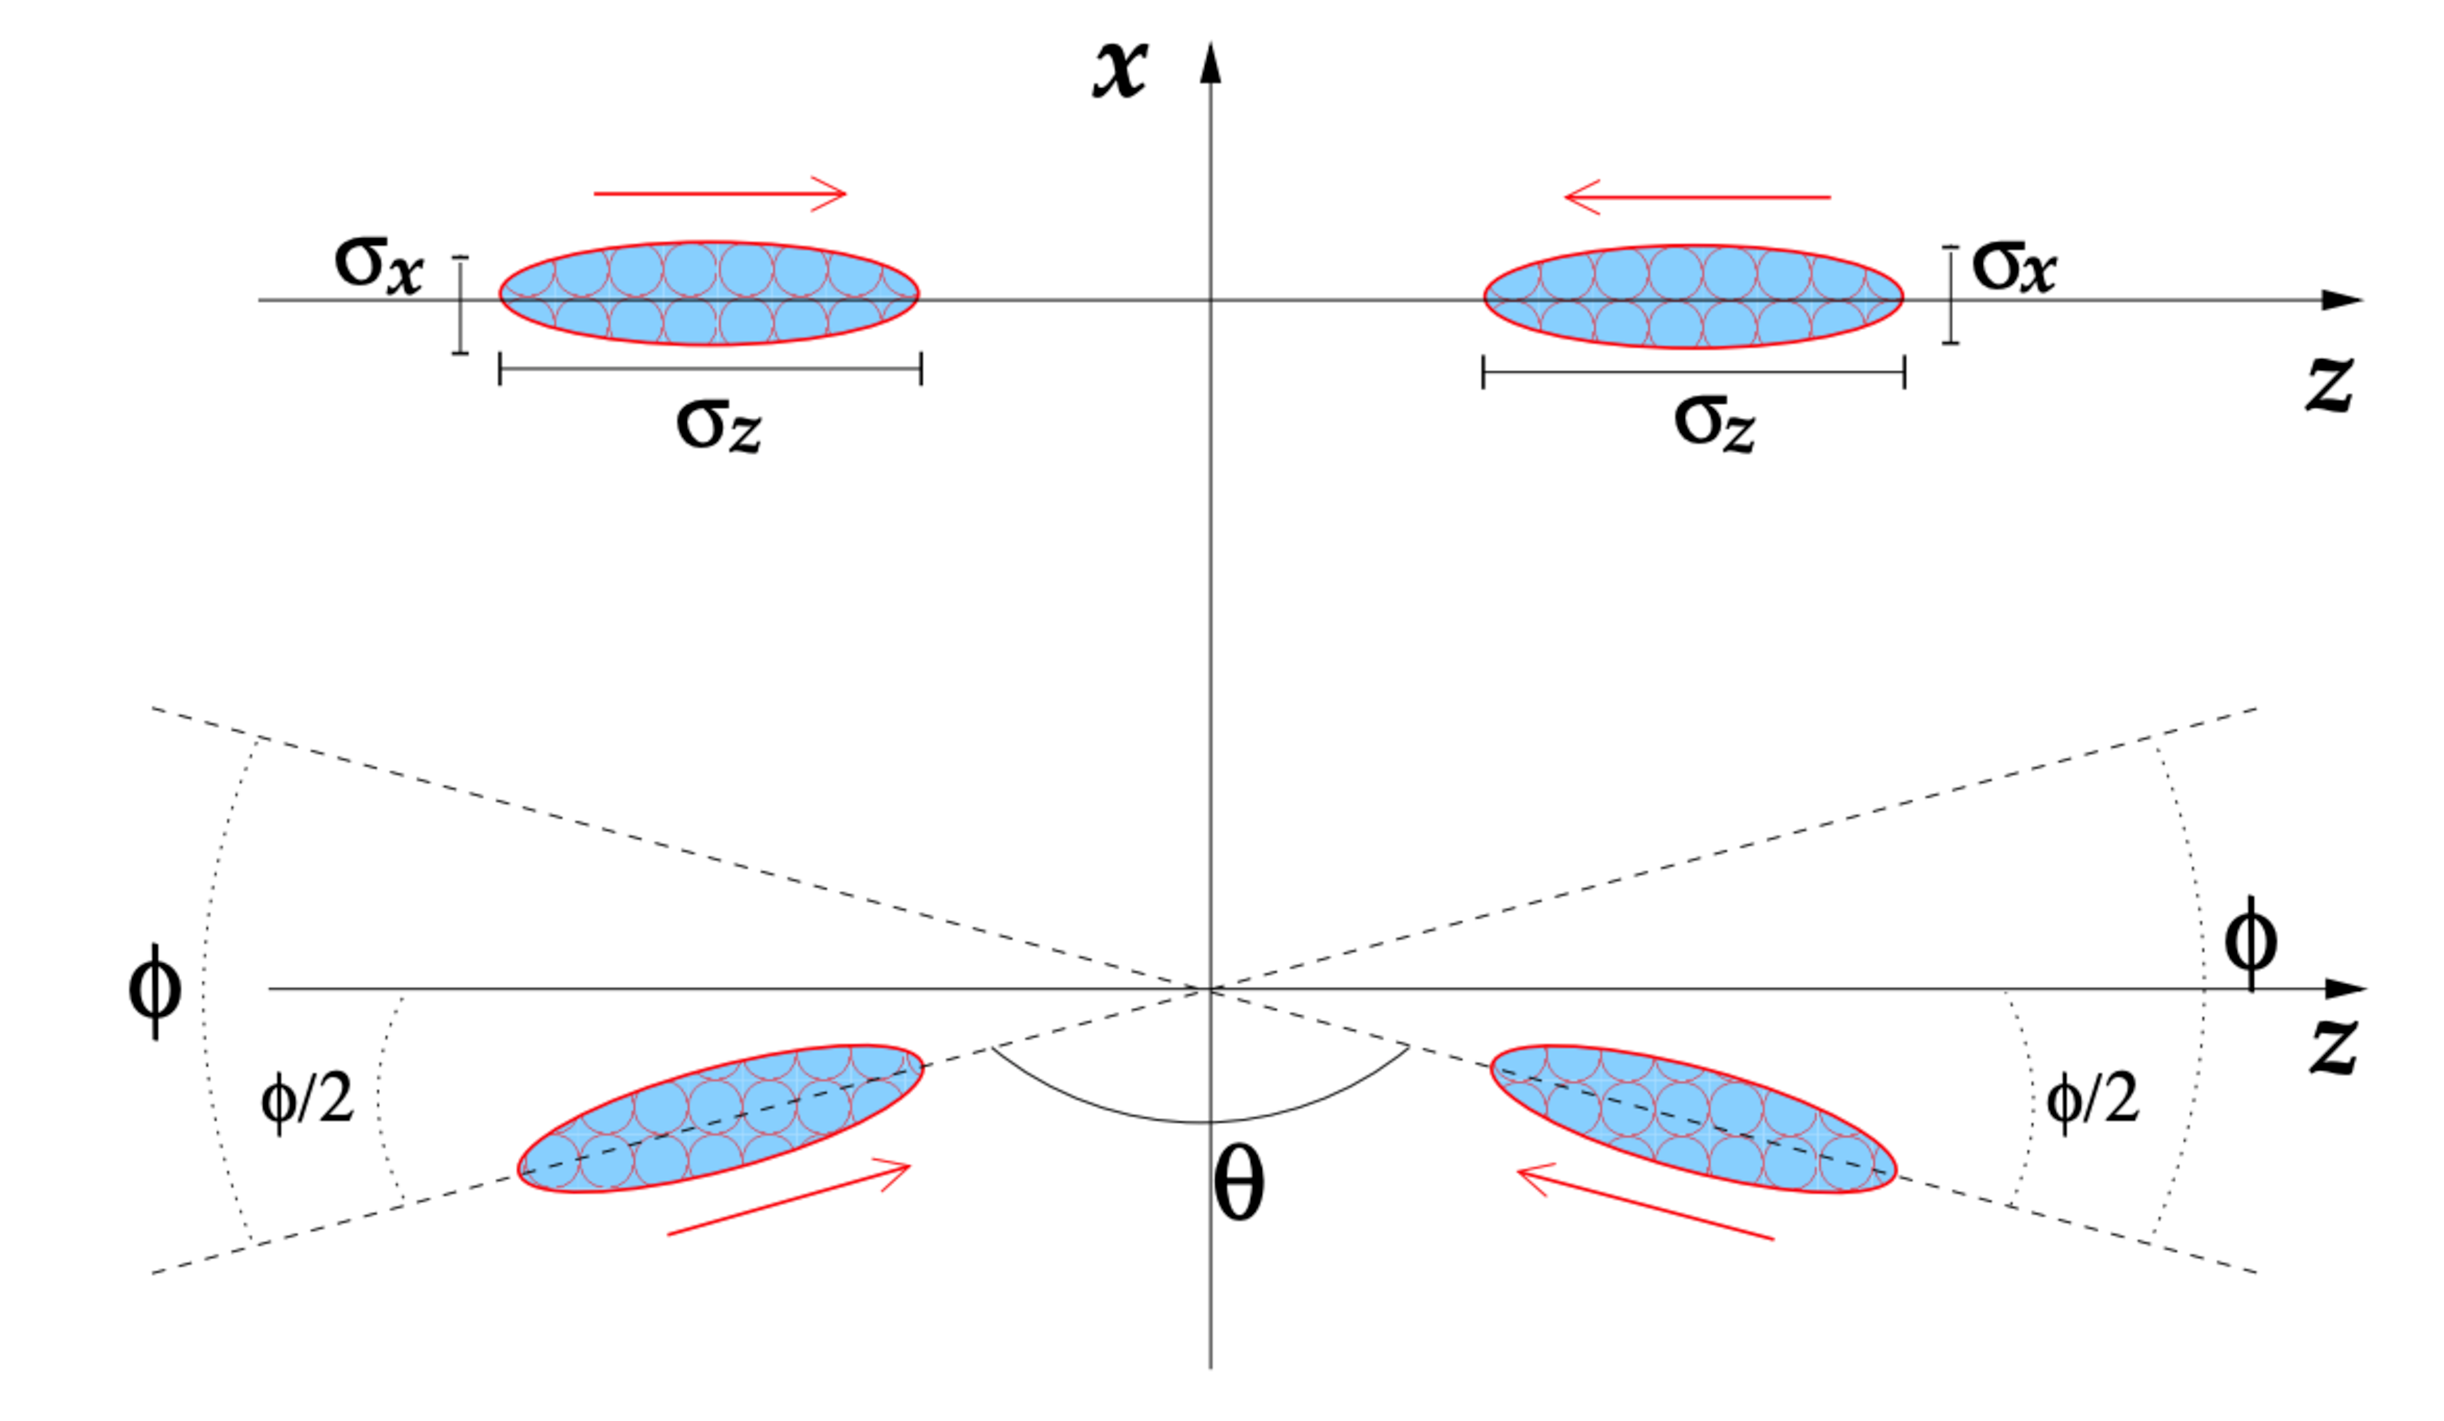
\includegraphics[width=0.6\textwidth]{chapters/2.detector/figs/beam_crossing.pdf}
  \caption{
    A digram showing the crossing of two proton bunches in the $x$\nobreakdash-$z$ plane in the case where the beams collide head on (above) and with a small crossing angle $\phi$ (below).
    %At the \LHC $\phi \approx \SI{285}{\radian}$.
    Reproduced from \cite{Cannoni:2016hro}.
  }
  \label{fig:beam_crossing}
\end{figure}
\end{comment}

The total luminosity recorded over the course of \runtwo is shown in \cref{fig:run2_lumi}. In total, \intlumi of usable physics data was collected over the three-year run.
The uncertainty on the total integrated luminosity is \pct{1.7} \cite{ATLAS-CONF-2019-021}.
%
\begin{figure}[!htbp]
  \centering
  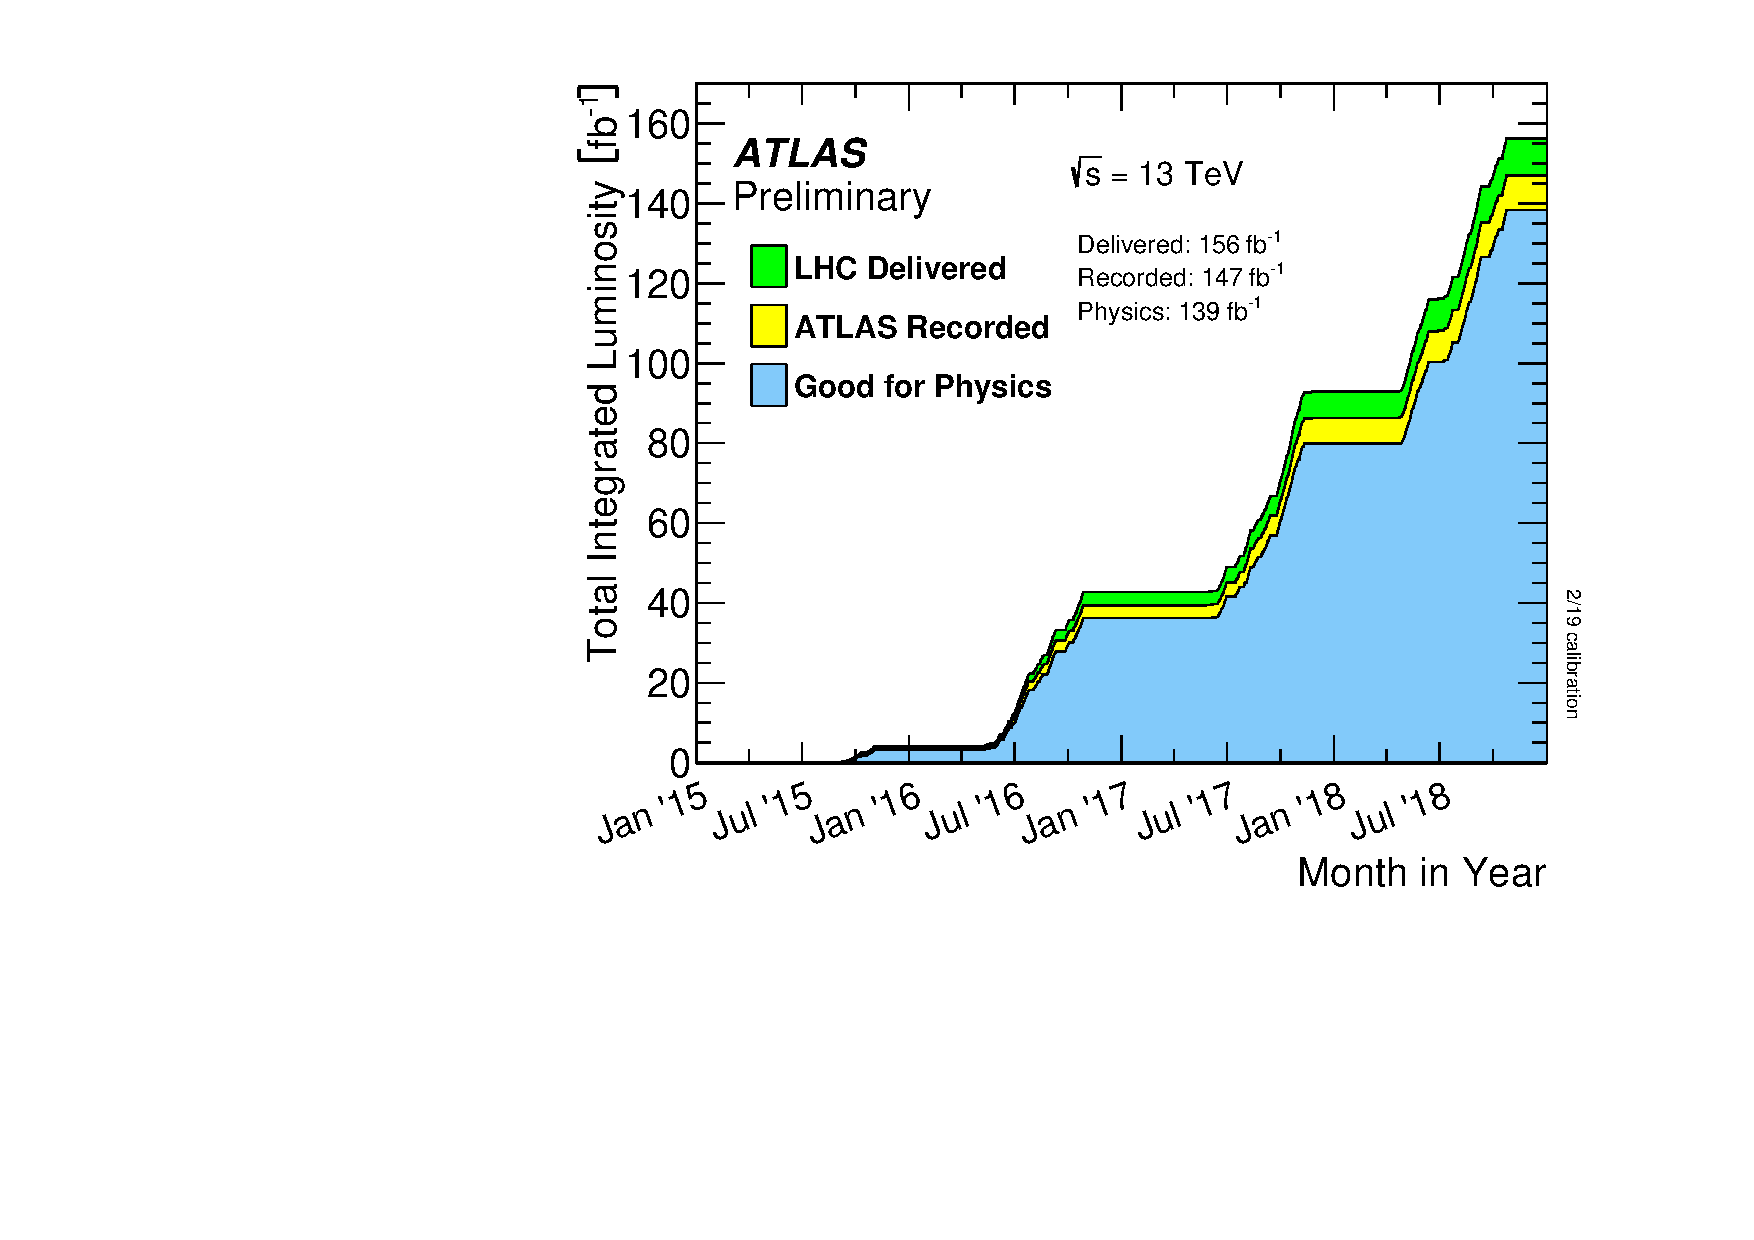
\includegraphics[width=0.6\textwidth]{chapters/2.detector/figs/intlumivstimeRun2DQall.pdf}
  \caption{
    Delivered, recorded, and usable integrated luminosity as a function of time over the course of \runtwo \cite{atlas-lumi-run2}.
    A total of \intlumi of collision data is labelled as good for physics, meaning all sub-detector systems were operating nominally.}
  \label{fig:run2_lumi}
\end{figure}
%


\subsubsection{Pile-up}

At the centre of the ATLAS detector, bunches of more than $10^{11}$ protonsare collided.
Each bunch-crossing is called an \textit{event}.
There is generally one hard proton-proton scatter per event.
Additional interactions are typically relatively soft (\lowpt) and are known as \textit{pile-up}.
%Pile-up complicates the reconstruction of the hard scatter event as results of the interactions of different proton-proton interactions have to be separated.
Pile-up from interactions within the same bunch-crossing is known as \textit{in-time} pile-up while residual signatures from previous bunch-crossings is known as \textit{out-of-time} pile-up.
The number of pile-up interactions is denoted $\mu$, which is often given as a time-averaged value \angles{\mu}.
Histograms showing the number of pile-up interactions over the course of \runtwo are shown in \cref{fig:run2_pile-up}.
%
\begin{figure}[!htbp]
  \centering
  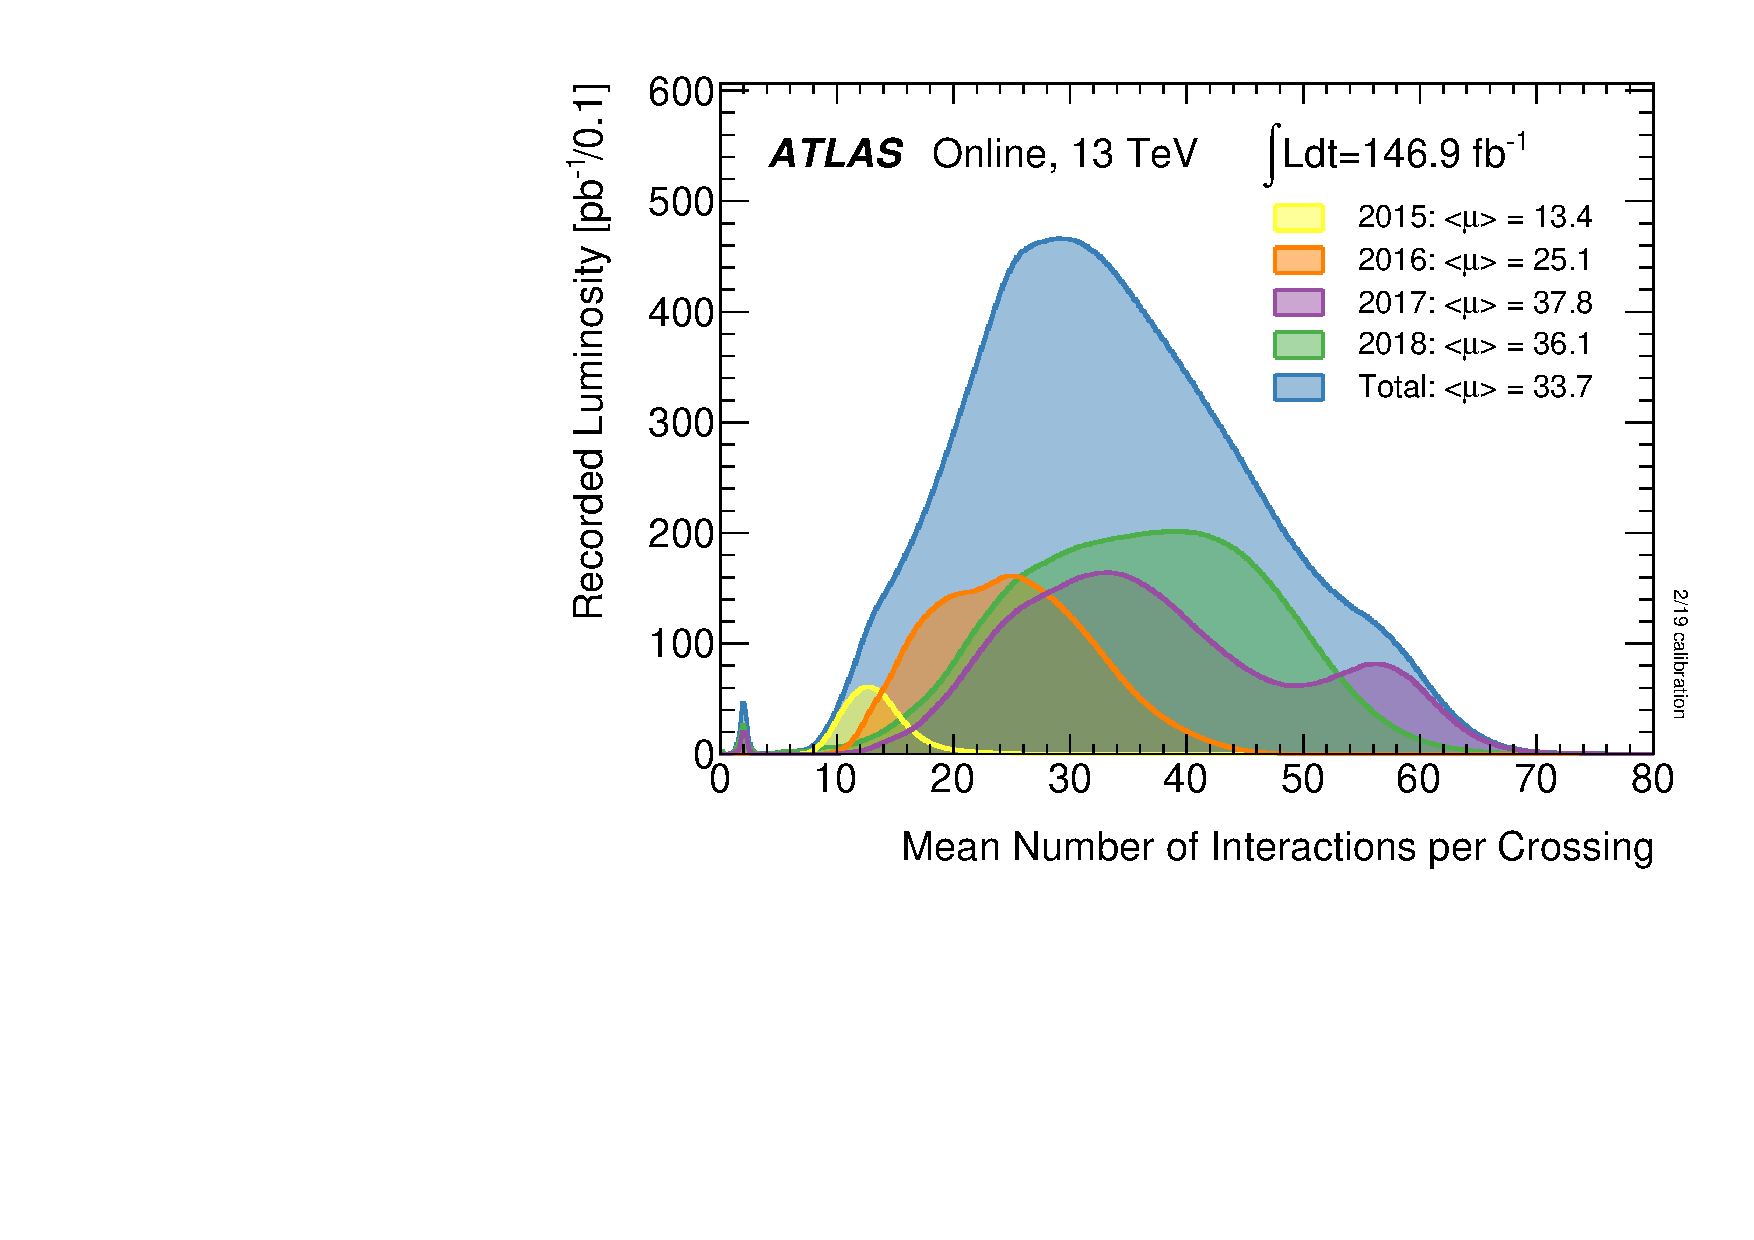
\includegraphics[width=0.6\textwidth]{chapters/2.detector/figs/mu_2015_2018.pdf}
  \caption{
    Average pile-up profiles measured by ATLAS during \runtwo \cite{atlas-lumi-run2}.
  }
  \label{fig:run2_pile-up}
\end{figure}
%


\section{The ATLAS Detector}\label{sec:atlas_detector}

The \ATLAS\footnote{\textbf{A} \textbf{T}oroidal \textbf{L}HC \textbf{A}pparatu\textbf{S}.} detector is made up of several specialised sub-detectors which are arranged concentrically around the nominal interaction point at the centre of the detector, as shown in \cref{fig:atlas_detector}.
The detector is designed to cover nearly the entire solid angle around the collision point.
In this section a brief overview of each sub-detector is given, in order of increasing radial distance from the point of collision.
The inner tracking detector is described in \cref{sec:atlas_id}, the electromagnetic and hadronic calorimeters in \cref{sec:atlas_calorimeter}, the muon spectrometer in \cref{sec:muon_spectrometer}, and finally the trigger is described in \cref{sec:trigger}.
More complete information on the detector can be found in \rcite{PERF-2007-01}, while an overview of physics performance is given in \cite{ATLAS-TDR-14}.

\begin{figure}[!htpb]
  \centering
  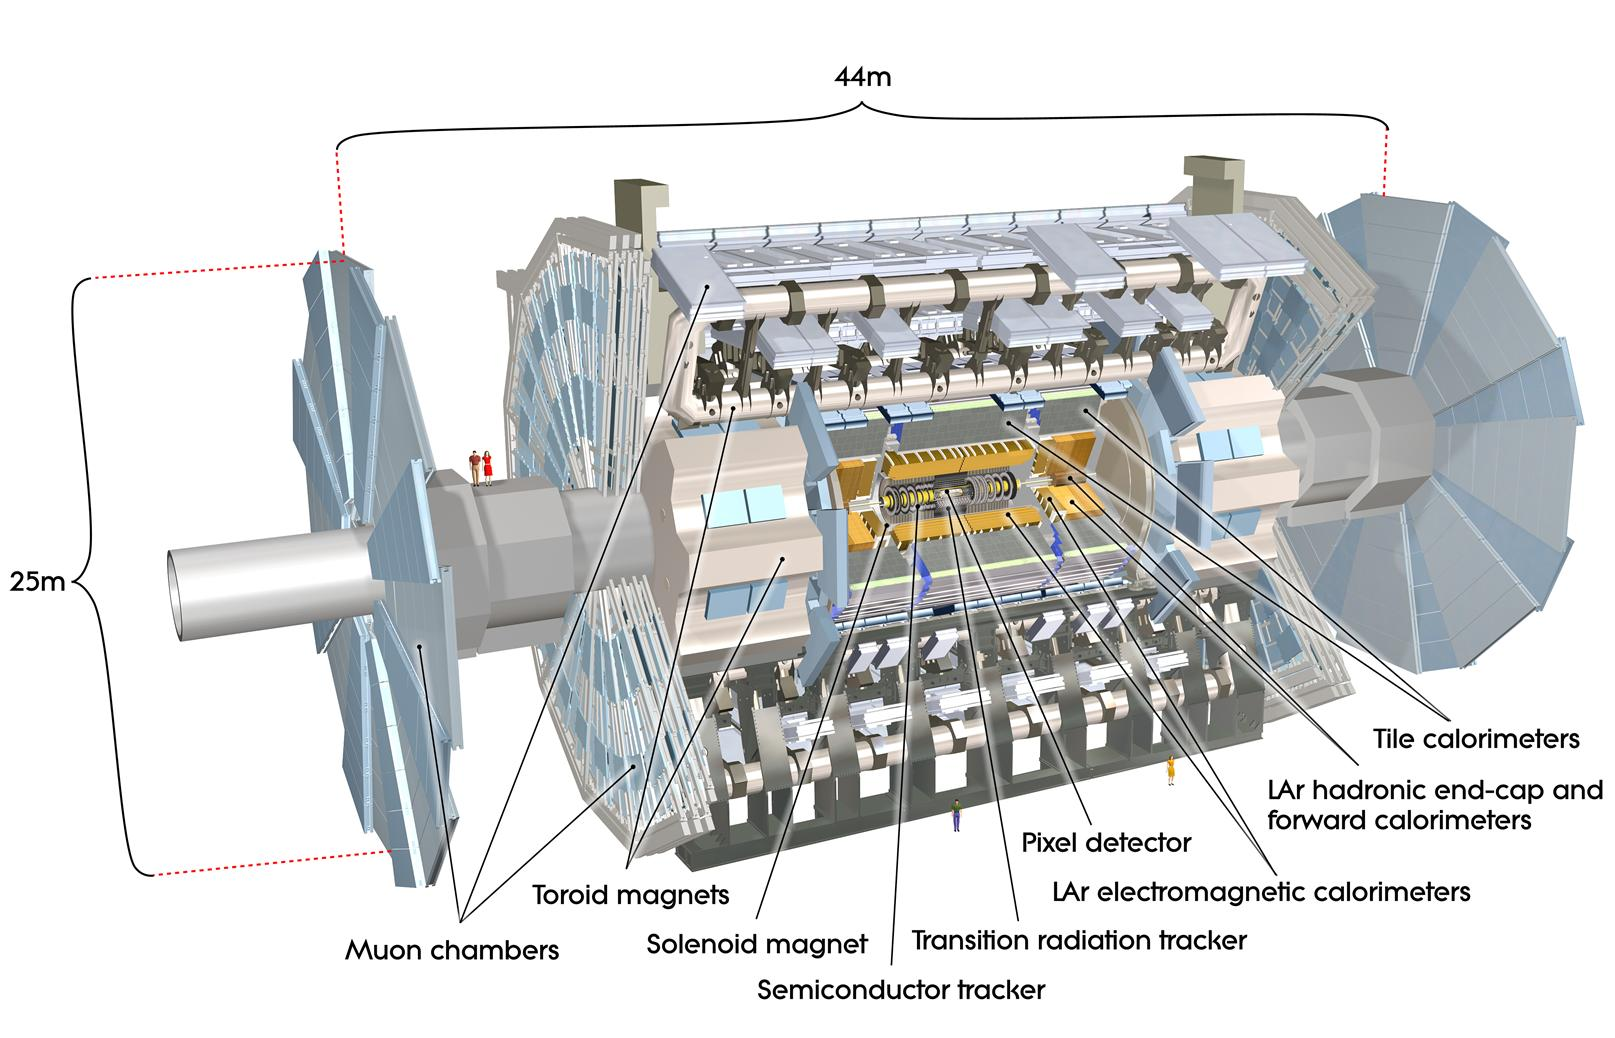
\includegraphics[width=0.9\textwidth]{chapters/2.detector/figs/atlas_detector.jpg}
  \caption{
    A 3D model of the entire \ATLAS detector \cite{Jon-And:1237407}.
    Cutouts to the centre of the detector reveal the different subdetectors which are arranged in concentric layers around the nominal interaction point.
  }
  \label{fig:atlas_detector}
\end{figure}


\subsection{Inner Detector}\label{sec:atlas_id}

The inner-detector system (ID) provides high-resolution charged particle trajectory tracking in the range $|\eta| < 2.5$.
The ID is immersed in a \SI{2}{\tesla} axial magnetic field, produced by a superconducting solenoidal magnet, which enables the measurement of particle momentum and charge.
After \runthree, the ID will be replaced by the ITk \cite{ATLAS-TDR-30,ATLAS-TDR-25}.

The inner detector is made up of several sub-systems, shown in \cref{fig:atlas_id_run1,fig:atlas_id_run2}.
The high-granularity silicon pixel detector covers the innermost region and typically provides four spacepoint measurements per track.
It is followed by the silicon microstrip tracker (SCT), which usually provides a further four spacepoint measurements (8 hits) per track.
These silicon detectors are complemented by the Transition Radiation Tracker (TRT),
which enables radially extended track reconstruction up to $|\eta| = 2.0$ and typically provides 33 (38) additional hits in the barrel (endcap). 


\begin{figure}[!htpb]
  \centering
  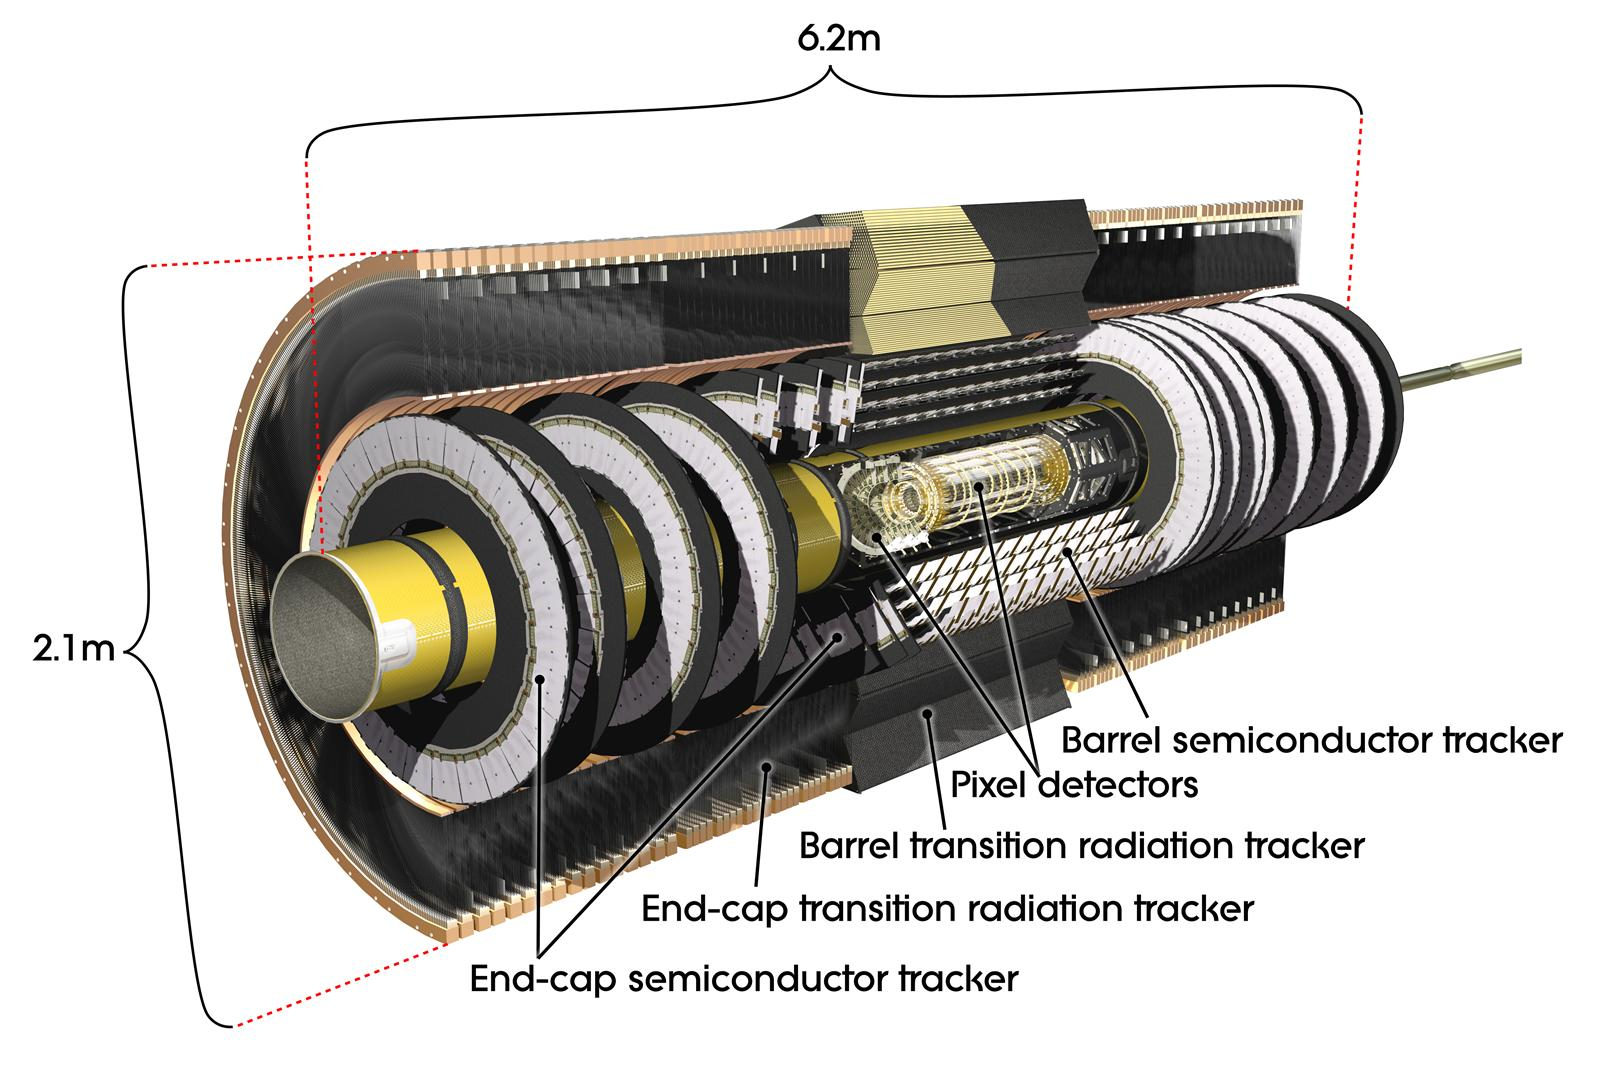
\includegraphics[width=0.75\textwidth]{chapters/2.detector/figs/atlas_id.jpg}
  \caption{
    A 3D model of the \ATLAS ID showing the pixel, SCT and TRT subdetectors \cite{atlasid}.
  }
  \label{fig:atlas_id_run1}
\end{figure}
%
\begin{figure}[!htpb]
  \centering
  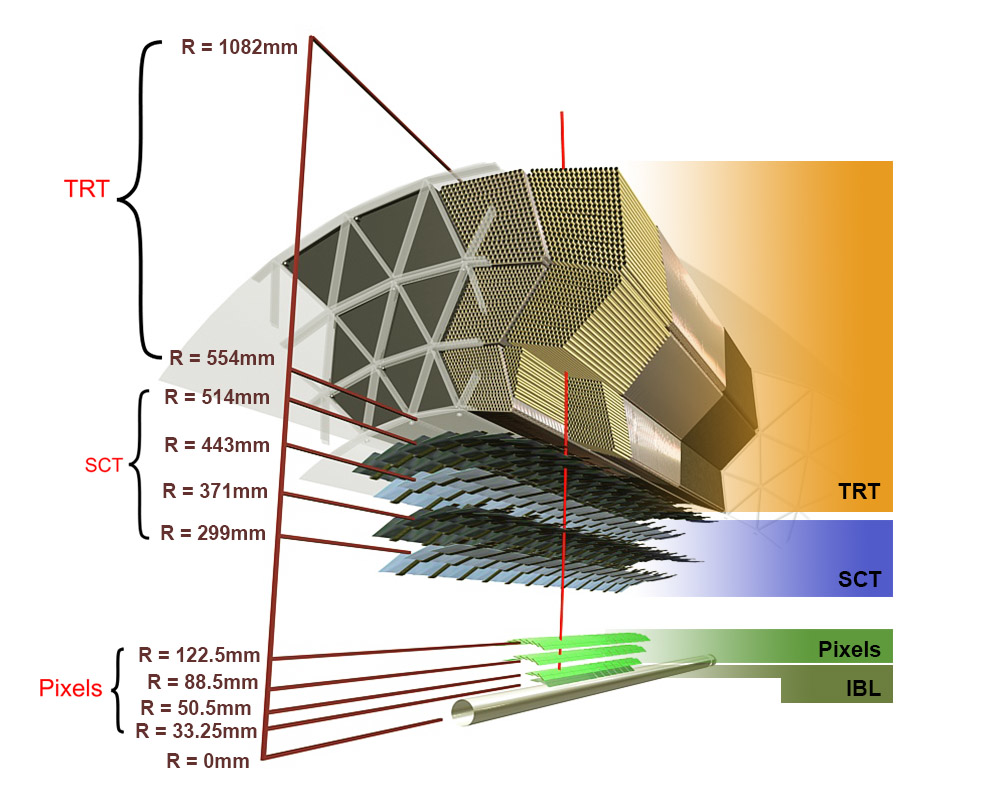
\includegraphics[width=0.75\textwidth]{chapters/2.detector/figs/atlas_id_xs.png}
  \caption{A cross-sectional view of the \ATLAS ID, with the radii of the different barrel layers shown \cite{atlastrackingdocs}.}
  \label{fig:atlas_id_run2}
\end{figure}
%

The target inverse momentum resolution for the combined ID measurement is parameterised as a function of the track transverse momentum and polar angle \cite{ATLAS-TDR-14}.
The parameterisation is given by
%
%\begin{equation}
%  \frac{\sigma_{\pt}}{\pt} = \pct{0.05} \pt \oplus \pct{1} .
%\end{equation}
\begin{equation}
  \sigma(1/\pt) = 0.36 \oplus \frac{13}{\pt \sin\theta} ~\SI{}{\per\TeV} ,
\end{equation}
%
where $\oplus$ denotes a sum in quadrature.
For \lowpt tracks (e.g. $\pt \approx \SI{500}{\MeV}$) in the central region this corresponds to a relative error of approximately \pct{0.01}.
Meanwhile for \highpt tracks (e.g. $\pt \approx \SI{100}{\GeV}$) in the central region this corresponds to a relative error of approximately \pct{4}.
The momentum resolution generally good enough to correctly identify the sign of the charge on particles up to the highest energies expected at the \LHC.
The transverse impact parameter resolution $\sigma(\dzero)$ is parameterised similarly as
%
\begin{equation}
  \sigma(\dzero) = 11 \oplus \frac{115}{\pt \sin\theta} \SI{}{\micro\meter} .
\end{equation}
%
Typical uncertainties for the transverse IP resolution are \SI{230}{\micro\meter} and \SI{11}{\micro\meter} for low and \highpt tracks in the central region, respectively.

\subsubsection{Pixel Detector}
The silicon pixel detector is comprised of four cylindrical barrels at increasing radii from the beamline, and four disks on each side.
The innermost barrel layer is the insertable B-layer (IBL), shown in \cref{fig:atlas_ibl}.
The IBL was installed before \runtwo \cite{ATLAS-TDR-19,PIX-2018-001} and lies approximately just \SI{33}{\milli\meter} from the beam axis.
The second-to-innermost layer is often referred to as the B-layer.
%Radiation-hard electronics are used to read out the 140 million channels.
The specification of the pixel detector determines the impact parameter resolution and the ability to reconstruct primary and secondary vertices.
The detector is required to have a high granularity (i.e. resolution) to maintain the low occupancy required to resolve nearby particles. %(high sparsity to resolve different tracks).
Individual pixels are \SI{50}{\micro\meter} in the transverse direction $R\phi$ and \SI{400}{\micro\meter} in the longitudinal $z$ direction (\SI{250}{\micro\meter} for the IBL).
Cluster positions have a resolution of approximately \SI{10}{\micro\meter} in $R\phi$ and \SI{100}{\micro\meter} in $z$.

%giving a resolution of 10 µm in the transverse direction and 115 µm in the longitudinal direction in the barrel region.
%For the IBL, pixels are \SI{50}{\micro\meter} in the $R\phi$ direction and \SI{250}{\micro\meter} in the $z$ direction, giving a cluster resolution of 10 µm in the transverse direction and 115 µm in the longitudinal direction in the barrel region.
%%Pixel clusters and provide an Xlocal resolution of about 10 µm, depending on the particle incident angle

\begin{figure}[!htpb]
  \centering
  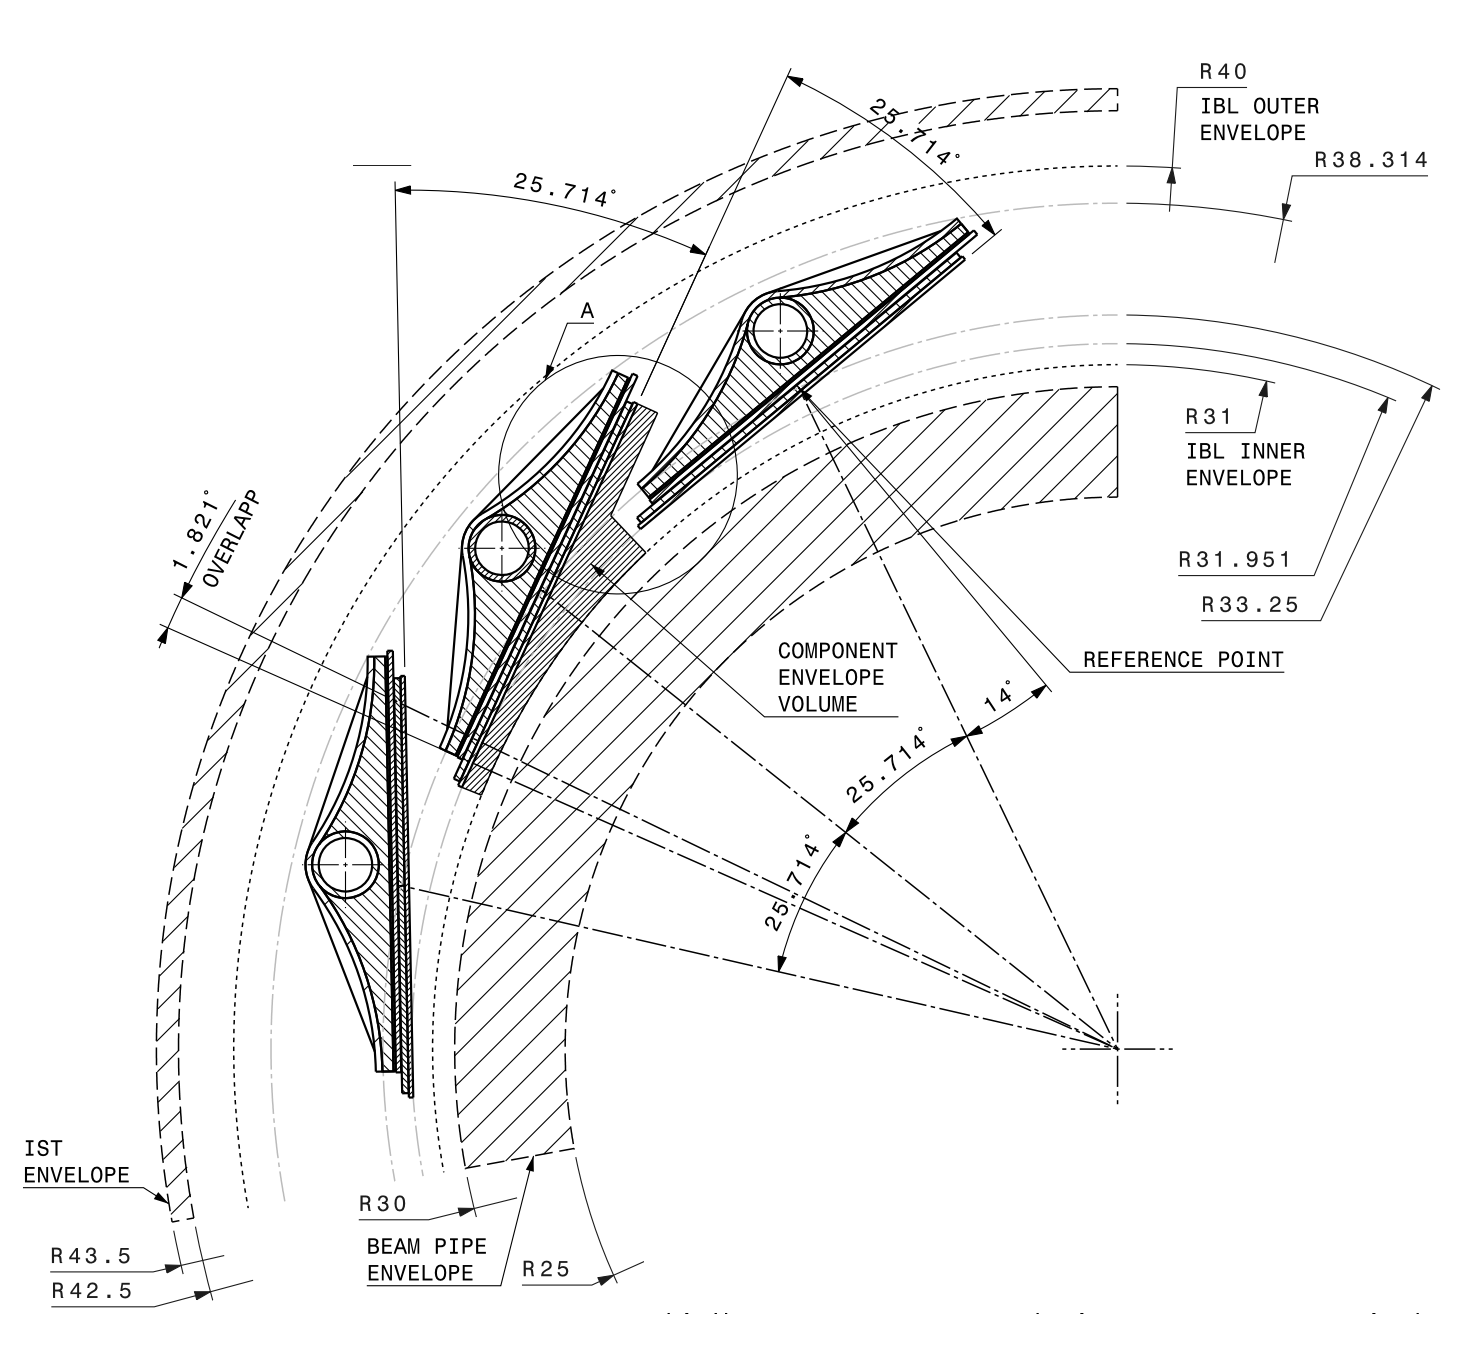
\includegraphics[width=0.6\textwidth]{chapters/2.detector/figs/atlas_ibl.png}
  \caption{A schematic cross-sectional view of the \ATLAS IBL \cite{ATLAS-TDR-19}.}
  \label{fig:atlas_ibl}
\end{figure}

\subsubsection{Semi-Conductor Tracker (SCT)}
The SCT is made up of four concentric barrel layers in the central region, and nine disks in each end-cap.
Each layer is itself made of a pair of silicon microstrip layers, with a small stereo angle (\SI{20}{\milli\radian}) between the two layers enabling the $z$\nobreakdash-coordinate to be measured from a pair of strip measurements.
The SCT typically provides four precision spacepoint measurements (eight strip measurements) per track in the barrel region.
These have intrinsic uncertainties of \SI{17}{\micro\meter} in the transverse direction $R\phi$, and \SI{580}{\micro\meter} in the longitudinal direction $z$ \cite{IDET-2013-01}.
The measurements provide a contribution to the measurement of charged particle momentum and impact parameter.
%The high granularity enables good pattern recognition
%Charge-particle tracks can be distinguished if separated by more than $\sim \SI{200}{\micro\meter}$.
%Hits are registered as binary signals if the pulse height in a channel exceeds a certain threshold.


\subsubsection{Transition Radiation Tracker (TRT)}
The TRT is a straw-tube tracker which complements the higher-resolution silicon-based tracks by offering a larger number of hits per track (typically more than 30) and a long lever arm, which aids the accurate measurement of particle momentum. 
It is made up of approximately \num{300000} drift tubes with a diameter of \SI{4}{\milli\meter} which are filled with an argon/xenon gas mixture.
The walls of each tube are electrically charged, and a thin conducting wire runs along the center.
When a charged particle traverses a tube, it ionises the gas and the resulting liberated electrons drift along the electric field to the wire, where an associated charge is registered.
In the barrel the straws run parallel to the \axis{z} and therefore the TRT only provides tracking information in $R\phi$. Straws are arranged radially in the end-caps. The resulting two-dimensional spacepoints have a resolution of approximately \SI{120}{\micro\meter}.
The spaces between the straws are filled with a polymer which encourages the emission of transition radiation, aiding electron identification.

%It allows the ID to reconstruct $V_0$s which are especially interesting in CP-violating $B$ decays.
%Electron identification capability is added by employing xenon gas to detect transition-radiation photons created in a radiator between the straws. In addition it provides additional discrimination between electrons and hadrons
% provides electron identification information based on the fraction of hits (typically 30 in total) above a higher energy-deposit threshold corresponding to transition radiation.
%may be emitted by highly relativistic charged particles as they traverse a material boundary. This effect depends on the relativistic factor γ = E/m and is strongest for electrons, 
%means it can be used for particle identification (section 6). Typical photon energies are 5–30 keV. These soft X-rays can be absorbed by Xe atoms, depositing additional energy in the gas and leading to significantly higher readout signals. Suc

%Within the radial space available, the straw spacing has been optimised for tracking at the expense of electron identification, which would be improved by a greater path length through the radiator material and fewer active straws. 


% TR is a form of electromagnetic radiation emitted when a charged particle passes through inhomogeneous media, such as a boundary between two different media. The probability that a particle emits radiation is given by it's $\gamma$ (Lorentz) factor (ie particle velocity). Electrons in general have higher Lorentz factors than eg. pions, as they are lighter than pions. In this way, the TRT discriminates between lighter and heavier particles.

\subsection{Calorimeters}\label{sec:atlas_calorimeter}

The calorimeter system measures the energy of incident particles over the range $|\eta| < 4.9$.
There are two main sub-systems: the electromagnetic calorimeter (ECal), which focuses on the measurement of electrons and photons, and the hadronic calorimeter (HCal), which measures the energy of hadrons.
A schematic view of the calorimeter system is shown in \cref{fig:atlas_calos}.
Upon entering the calorimeter, incident particles will interact with the detector material to produce a shower of secondary particles with reduced energies. 
The charge deposited in this process is measured to reconstruct the energy of the initial incident particle.
The two calorimeter sub-systems must provide strong containment of showering particles to prevent punch-through of EM and hadronic particles to the HCal and muon systems respectively.


%the fine granularity of the EM calorimeter is ideally suited for precision measurements of electrons and photons. The coarser granularity of the rest of the calorimeter is sufficient to satisfy the physics requirements for jet reconstruction and $E_T^{\textrm{miss}}$ measurements.     

%A narrow transverse profile is characteristic of an electromagnetic cascade. Hadrons passing through matter also initiate cascades through inelastic hadron-nuclei interactions. The shower produces secondary hadrons and leptons and has a comparatively wide transverse profile. 

%Nuclear interaction length is the mean distance travelled by a hadronic particle before undergoing an inelastic nuclear interaction.
%The nuclear interaction length is about an order of magnitude greater than the radiation length of the material. Therefore, like most general purpose experiments, ATLAS uses two different calorimetry systems to measure electrons and photons (the ECal) and hadrons (the HCal). 

%
\begin{figure}[!htpb]
  \centering
  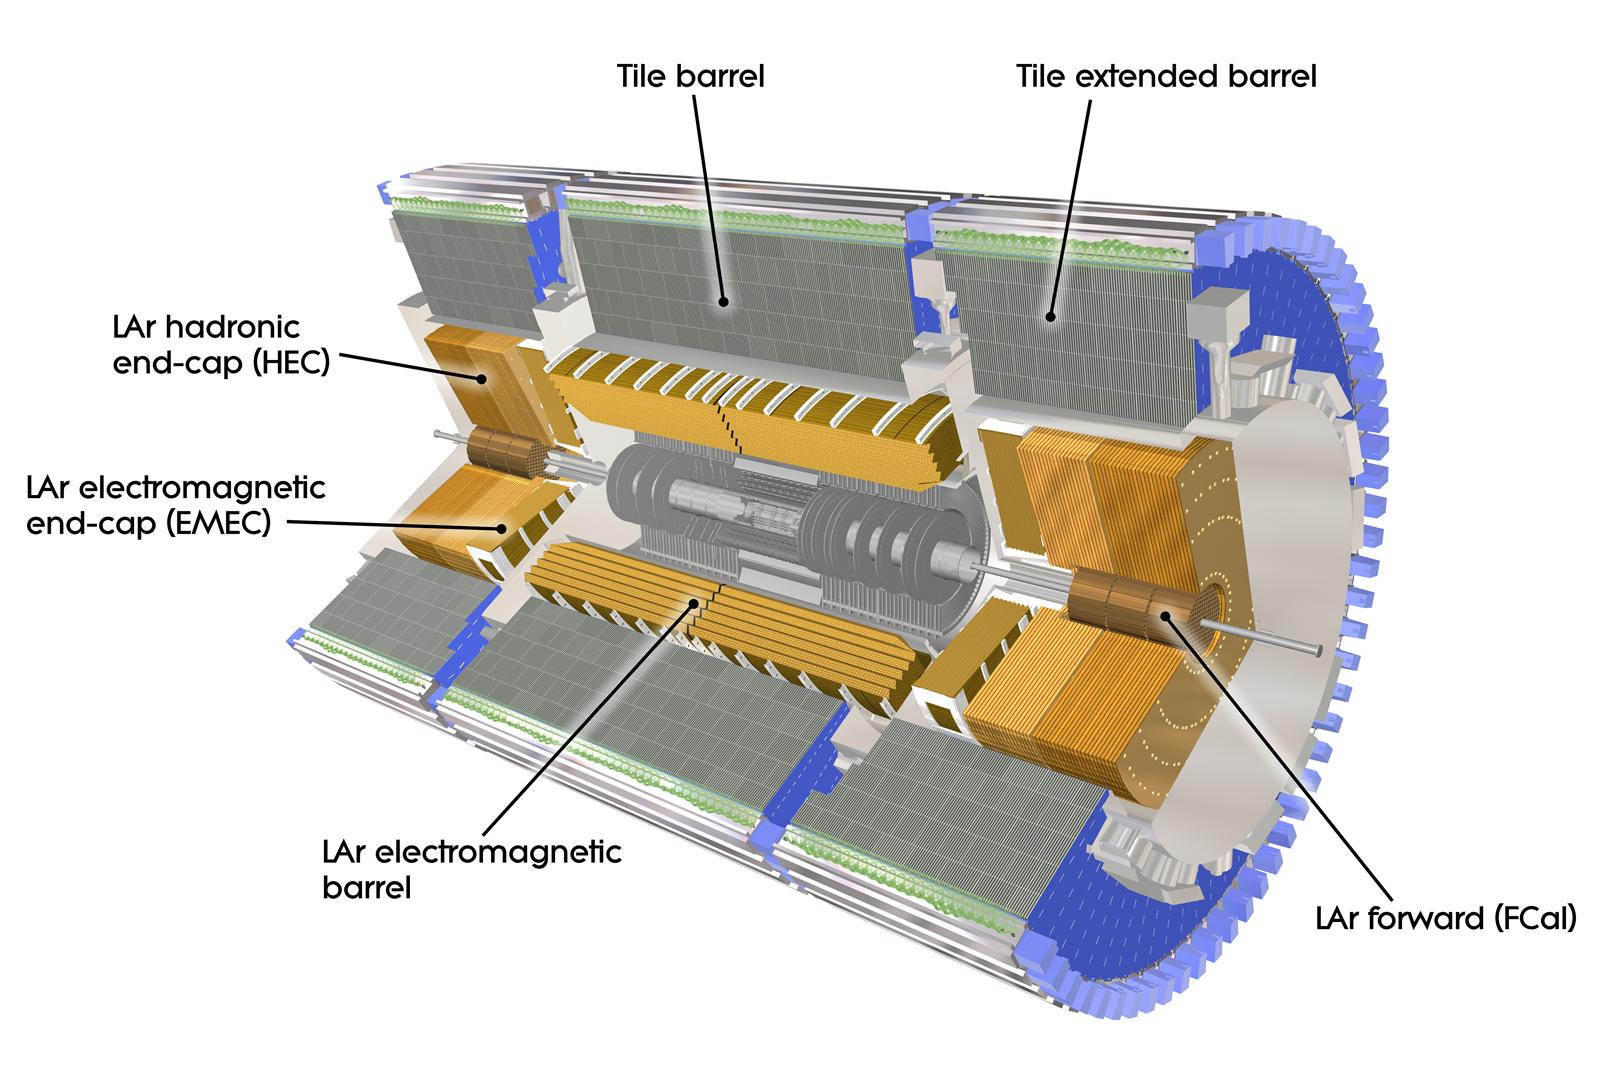
\includegraphics[width=0.8\textwidth]{chapters/2.detector/figs/atlas_calos.jpg}
  \caption{
    The \ATLAS calorimeters \cite{atlascalo}.
    The ECal uses LAr-based detectors, while the HCal uses mainly scintillating tile detectors.
    In the forward region the HCal also includes the LAr hadronic endcaps.
  }
  \label{fig:atlas_calos}
\end{figure}
%


\subsubsection{Liquid Argon (LAr) Electromagnetic Calorimeter}
The more granular lead/liquid-argon ECal covers the region $|\eta|< 3.2$ and is split into barrel (covering $|\eta| < 1.475$) and end-cap (covering $1.375 < |\eta| < 3.2$) regions.
EM calorimetry works by encouraging electrons and photons to interact with electrically charged particles in detector material via bremsstrahlung ($e \rightarrow e\gamma$) and pair production ($\gamma \rightarrow e^+ e^- $).
The EM calorimeter uses lead absorber plates to initiate EM showers, resulting in secondary particles which ionise the surrounding liquid argon.
The charge is collected on copper electrodes and read out.
The accordion geometry of the ECal allows for a full coverage in $\phi$ without any azimuthal cracks.

The energy resolution of the LAr calorimeter is made up of a sampling and a constant term, which are summed in quadrature to produce the overall energy resolution.
The sampling term contributes approximately $\pct{10} / \sqrt{E}$, while the constant term adds an additional \pct{0.7}.
Photons with moderate transverse energy $\ET \approx \SI{50}{\GeV}$ have an overall energy resolution of at most \pct{1.6} over most of the pseudorapidity range.
At lower $\ET \approx \SI{10}{\GeV}$, the resolution is degraded to approximately \pct{5}.
The resolution measurements are obtained from test beam data \cite{ATLAS-TDR-14}.

%it initiates an electromagnetic cascade,
%The fine granularity of the EM calorimeter
%Additionally, multiple samplings of the shower are used to resolve its pointing vector.

\subsubsection{Hadronic Tile Calorimeter}
In the central barrel region with $|\eta| < 1.7$, the HCal uses a tile calorimeter with steel as an absorbing material, and scintillating tiles as the active material.
Two copper/liquid-argon calorimeter end-caps are also used.
Incident hadrons interact via the strong and electromagnetic forces with the absorber material, mainly loosing energy due to multiple inelastic nuclear collisions.
The active material captures the resulting electrons and photons to measure the energy of the incident hadron.

The hadronic energy resolution of the HCal is parameterised as a function of the hadron's transverse energy
%
\begin{equation}
  \sigma(\ET) / \ET = \pct{50} / \sqrt{\ET} \oplus \pct{3} ,
\end{equation}
%
corresponding to a energy resolution of \pct{11} (\pct{6.5}) for a hadron with \ET of approximately \SI{10}{\GeV} (\SI{50}{\GeV}) \cite{ATLAS-TDR-03}.

%Hadrons are relatively massive and cannot radiate much of their energy through bremsstrahlung, and they lose their energy mainly through multiple nuclear collisions.  Hadrons passing through matter also initiate cascades through inelastic hadron-nuclei interactions.

%The tile calorimeter is placed directly outside the EM calorimeter envelope.o 
%The barrel covers the region -1.0<η<1.0, and the extended barrels cover the region 0.8<|η|<1.7.

%LAr hadronic end-cap calorimeter (HEC). Located directly behind (in $z$) the end-cap electromagnetic calorimeter and sharing the same LAr cryostats. The high level of radiation in the forward regions would cause severe damage to plastic scintillators. In the end-caps, parallel copper plates are submerged in liquid argon, which is preferred as the active medium because of its inherent radiation hardness.


\subsection{Muon Spectrometer}\label{sec:muon_spectrometer}

Due to their higher mass, muons easily pass unimpeded through the ID and calorimeters and therefore require specialised detectors for their measurement.
% higher mass means brem is less effective at slowing them down. though
The Muon Spectrometer (MS) is made up of dedicated tracking and triggering hardware, as shown in \cref{fig:atlas_muon_system}.
The precision tracking system uses three layers of monitored drift tubes with a barrel region covering $|\eta| < 1.2$ and end-caps covering $1 < |\eta| < 2.7$. The inner layers of the end-caps use cathode strip chambers to better cope with the high occupancy in the forward region.
The trigger system is comprised of resistive plate chambers in the barrel region covering $|\eta| < 1.0$ and thin gap chambers in the end-cap regions covering $1 < |\eta| < 2.4$.
A set of three superconducting air-core toroidal magnets, each made up of eight coils, is used in each of the barrel and end-caps to deflect the muons as the pass through the MS, allowing their momentum and charge to be measured from the direction and magnitude of curvature.
The toroidal magnets generate a field which is largely orthogonal to the muon trajectories which allows for maximum deflection.
The transverse momentum resolution (measured for combined ID and muon tracks, see \cref{sec:lepton_reco}) has been measured to be approximately \pct{1.7} in the central region for \lowpt muons, increasing to \pct{4} for \highpt muons in the forward regions \cite{Artoni:1953654}.
%
\begin{figure}[!htpb]
  \centering
  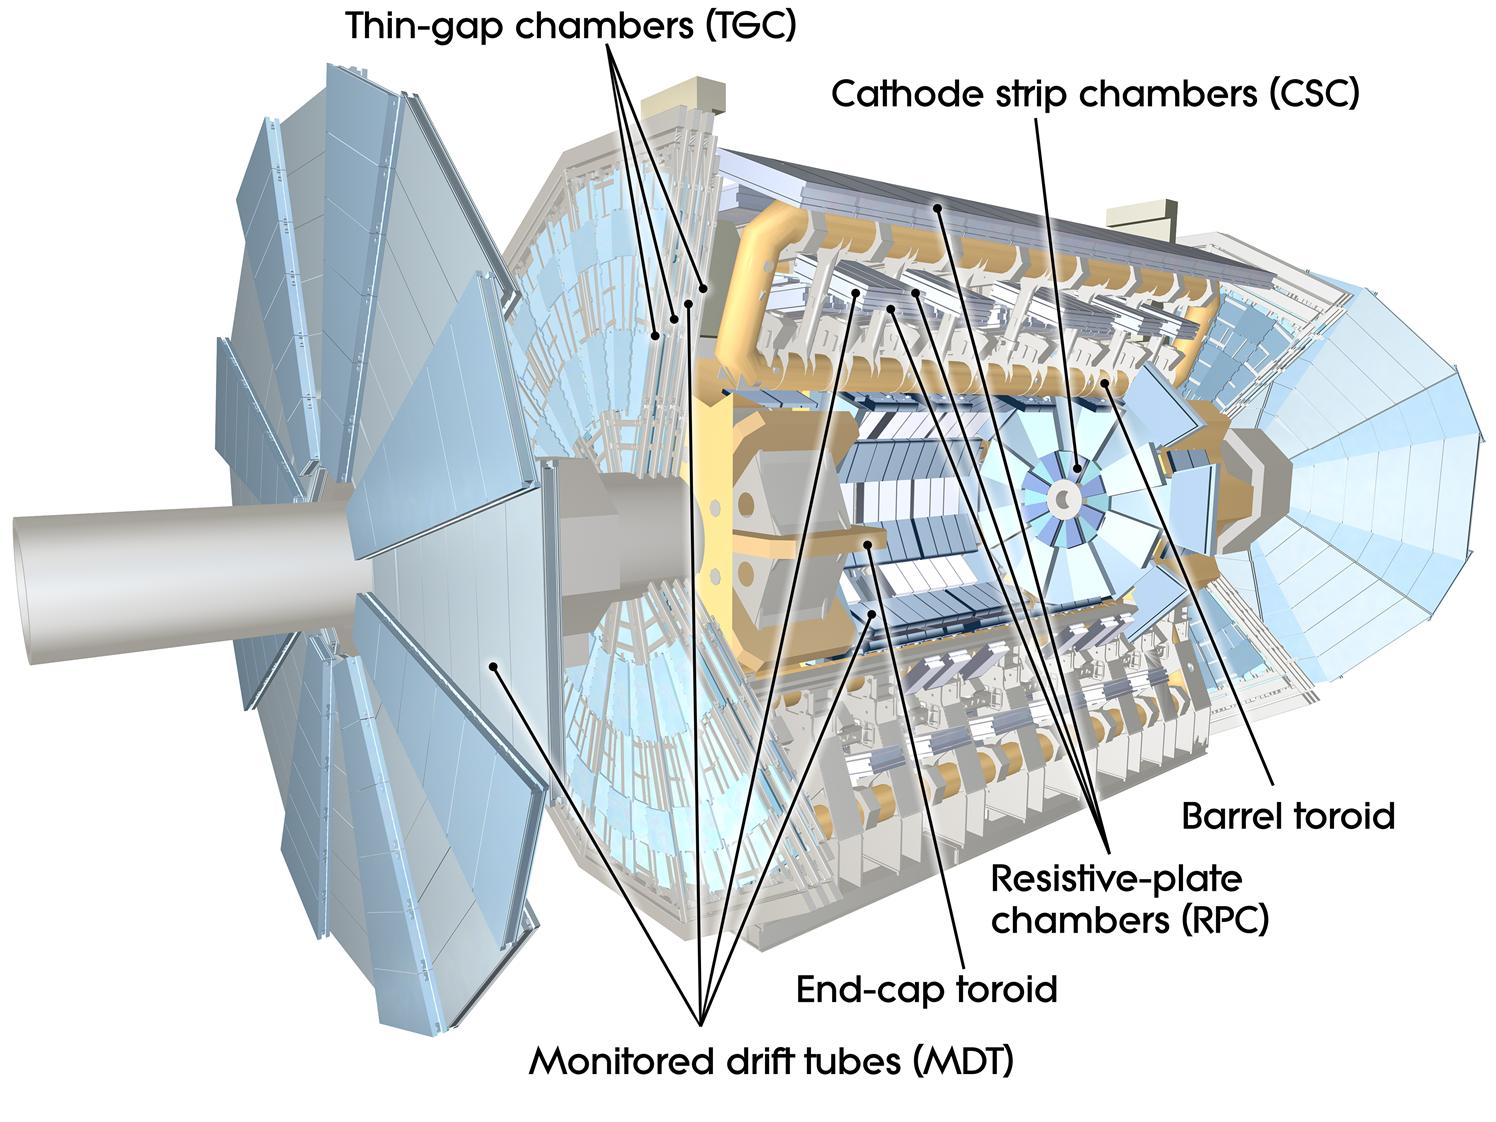
\includegraphics[width=0.7\textwidth]{chapters/2.detector/figs/atlas_muon_system.jpg}
  \caption{The \ATLAS muon spectrometer \cite{atlasmuon}.}
  \label{fig:atlas_muon_system}
\end{figure}
%


\subsection{The Trigger}\label{sec:trigger}
The \SI{25}{\nano\second} bunch spacing used over the course of \runtwo corresponds to a bunch-crossing or event rate of \SI{40}{\mega\hertz} (see \cref{tab:lhc_runs}).
If the full information for the detector was written out for each event, this would correspond to the generation of \SI{60}{\tera\byte} of data each second.
This is more than can be feasibly read out from the hardware, processed and stored, requiring the use of a trigger system which quickly makes a decision about whether or not an event is potentially interesting and should be kept for further analysis.
The trigger system is comprised of two levels which aim to identify various signatures, such as electrons, muons, taus, photons, and jets (including \bjets), as well as events with large total or missing transverse energy.
The hardware-based Level-1 (L1) trigger uses coarse information from the calorimeters and MS to accept events at an average rate of \SI{100}{\kilo\hertz} approximately \SI{2.5}{\micro\second} after the event.
After the L1 trigger, the software-based High Level Trigger (HLT) makes use of \num{40000} CPU cores to make a final selection on surviving events in approximately a few hundred milliseconds. 
The final event read-out rate is approximately \SI{1.2}{\kilo\hertz}, corresponding to \SI{1.2}{\giga\byte\per\second} of permenant data storage.
More information is provided in \cite{TRIG-2016-01}.
%Regions of Interest (ROIs) from the L1 trigger are used.

%The L1 trigger searches for high transverse-momentum muons, electrons, photons, jets, and $\tau$-leptons decaying into hadrons, as well as large missing and total transverse energy. Its selection is based on information from a subset of detectors. High transverse-momentum muons are identified using trigger chambers in the barrel and end-cap regions of the spectrometer. Calorimeter selections are based on reduced-granularity information from all the calorimeters. Results from the L1 muon and calorimeter triggers are processed by the central trigger processor, which implements combinations of different trigger selections. In each event, the L1 trigger also defines one or more Regions-of-Interest (RoI’s), i.e. the geographical coordinates in $\eta$ and $\phi$, of those regions within the detector where its selection process has identified interesting features. The RoI data include information on the type of feature identified and the criteria passed, e.g. a threshold. This information is subsequently used by the high-level trigger.

%The L2 selection is seeded by the RoI information provided by the L1 trigger. L2 selections use, at full granularity and precision, all the available detector data within the RoI’s (approximately 2\% of the total event data). The L2 menus are designed to reduce the trigger rate to approximately 3.5 kHz, with an event processing time of about 40 ms, averaged over all events. The final stage of the event selection is carried out by the event filter, which reduces the event rate to roughly 200 Hz. Its selections are implemented using offline analysis procedures within an average event processing time of the order of four seconds.










\section{Reconstructed Physics Objects}\label{sec:physics-objects}

Event reconstruction is the process of analysing the output from the detector to determine the type and properties of particles present in an event. 
The reconstructed event provides information about the underlying physics process that led to these observable final state particles.
Events passing the trigger selection (described in \cref{sec:trigger}) undergo offline reconstruction, which makes use of the full information from the detector.
Reconstruction and analysis of events relies on the extensive \ATLAS software stack, see \rcite{ATL-SOFT-PUB-2021-001} for more information.

Several different reconstructed objects are used for physics analyses.
Objects relevant to this thesis are described below.



\subsection{Tracks}\label{sec:track_reco}
% diagram at 
% https://atlassoftwaredocs.web.cern.ch/trackingTutorial/idoverview/
The reconstructed trajectories of charged particles are referred to as \textit{tracks}.
Tracks are reconstructed from the energy depositions (called \textit{hits}) left by the particles as they traverse the the inner detector.
Tracks are used in the reconstruction of other objects, including vertices and jets, so their accurate reconstruction is a critical task.
A comprehensive introduction to ATLAS tracking is available in \rcite{Cornelissen:2007vba}, while specific optimisations for dense environments are detailed in Refs.~\cite{ATL-PHYS-PUB-2015-006, PERF-2015-08}.
An overview of track reconstruction is given below.

%Tracking is useful for: impact parameter measurements, vertexing for heavy-flavour and $\tau$ tagging.

\subsubsection{Space-point Formation (Clustering)}
When a charged particle traverses a silicon layer, charge can be collected in more than one pixel or strip.
This is due to the incident angle of the particles with respect to the sensor, and also the drift of electrons between sensors caused by the magnetic field.
Clusters (also called \textit{hits} or \textit{space-points}) are formed by clustering neighbouring pixels or strips and estimating locations of space-points using the shape and energy distribution of the clusters.

\subsubsection{Track Finding}
Space-points are used to build track seeds. These are groups of three hits which are geometrically compatible with being part of a track segment.
A combinatorial Kalman filter (KF) is used to build track candidates by extending track seeds.
The filter can create multiple track candidates per seed, with bifurcations along the track occurring when more than one compatible space-point exists on a given layer.
In this way, the KF creates an excess of \textit{track candidates}, which are only required to satisfy basic quality requirements. 
Track candidates are allowed to reuse or \textit{share} hits freely (a single hit may be used by multiple track candidates).
Typically, the presense of shared hits is a predictor of a bad track due to the high granularity of the ATLAS tracking detectors.
At this stage, there can also be a large number of incorrect hits assigned to otherwise good tracks, and additionally large numbers of \textit{fake} tracks, which are comprised of a majority of wrong hits and do not correspond to the trajectory of any one physical particle (fake tracks are defined as those where the majority of associated hits do not originate from one single truth particle, see \cref{eq:tmp_def}).
The low quality of tracks at this stage necessitates an ambiguity solving step, in which candidates are cleaned, and the highest quality track are selected.

\subsubsection{Ambiguity Solving}
Ambiguity solving was introduced as part of the ATLAS New Tracking effort \cite{Cornelissen:2007vba}, which was intended to improve track reconstruction performance in dense environments.
In the ambiguity solver, track candidates are processed individually in descending order of a track score. The track score quantifies the likelihood of the track corresponding to the trajectory of a real particle. Scoring uses a number of variables, including the number and positions of hits (preferring hits in more precise regions of the detector), the transverse momentum of the track and the track fit quality. The track fit quality describes the quality of the track as the $\chi^2$ divided by the number degrees of freedom on the track. A preference for high transverse momentum tracks promotes the successful reconstruction of the more physically interesting energetic particles, and suppresses the large number of wrong hits assigned to low momentum tracks.
The ambiguity solver also penalises tracks with missing hits on the innermost detector layers. 

During the processing of a track candidate, the track is cleaned (whereby problematic hits are removed), and, if the resulting track satisfies the quality selection criteria, a high precision fit of the track parameters using the surviving hits is performed.
The high precision fit makes full use of all available information, and uses an updated position and uncertainty estimate for each cluster obtained from a Neural Network (NN) \cite{PERF-2012-05}.
If the track has reached this stage without being rejected by passing various quality requirements, it is re-scored and returned to the list of track candidates.
If the same track is then processed again without requiring modification, it is added to the final track collection.
Track candidates that fall below certain quality threshold are rejected.
This selection does allow for the possibility of a track having small number of shared hits, as detailed in \cref{tab:fake_track_mva_selections}.

\begin{table}[!htbp]
  \footnotesize\centering
  \setlength{\tabcolsep}{0.5em} % for the horizontal padding
  \begin{tabular}{ll}
    \toprule\hline
    \textbf{Parameter} & \textbf{Selection} \\
    \hline
    $\pt$                & $> 500$ MeV \\
    $|\eta|$             & $<2.5$ \\
    $|\dzero|$           & $< 3.5$ mm \\
    $|\zzero\sin\theta|$ & $< 5$ mm \\
    Silicon hits         & $\ge 8$ \\
    Shared silicon hits  & $< 2$ \\
    Silicon holes        & $< 3$ \\
    Pixel holes          & $< 2$ \\
    \hline\bottomrule
  \end{tabular}
  \caption{
    Quality selections applied to tracks,
    where \dzero is the transverse IP of the track, \zzero is the longitudinal IP with respect to the PV and $\theta$ is the track polar angle (see \cref{sec:track_parameterisation} for the IP definitions).
    Silicon hits are hits on the pixel and SCT layers.
    Shared hits are hits used on multiple tracks which have not been classified as split by the cluster-splitting neural networks~\cite{PERF-2015-08}.
    %Shared hits on pixel layers are given a weight of 1, while shared hits in the SCT are given a weight of 0.5.
    A hole is a missing hit, where one is expected, on a layer between two other hits on a track.
    }% https://twiki.cern.ch/twiki/bin/view/AtlasProtected/TrackingCPRecsRun2R22#Selection_Criteria
  \vspace{4mm}
  \label{tab:fake_track_mva_selections}
\end{table}


\subsubsection{Neural Network Cluster Splitting}
As part of track cleaning, shared hits are classified by a NN to determine if they are compatible with the characteristic features of a merged cluster \cite{PERF-2012-05, ATL-PHYS-PUB-2015-006}.
A merged cluster is one made up of a combination of energy deposits from more than one particle, which have become merged due to the closeness of the associated particles and the limited resolution of the detector.
It is common for clusters to become merged in dense environments, as discussed in \cref{sec:b_had_reco}.
If the cluster is predicted to be merged it is labelled as being freely shareable, or \textit{split}.
Hits not compatible with the merged hypothesis can still be shared by a limited number of tracks, but come with a penalty for the track which may hinder its acceptance into the final track collection.
%
\begin{figure}[ht]
    \centering
    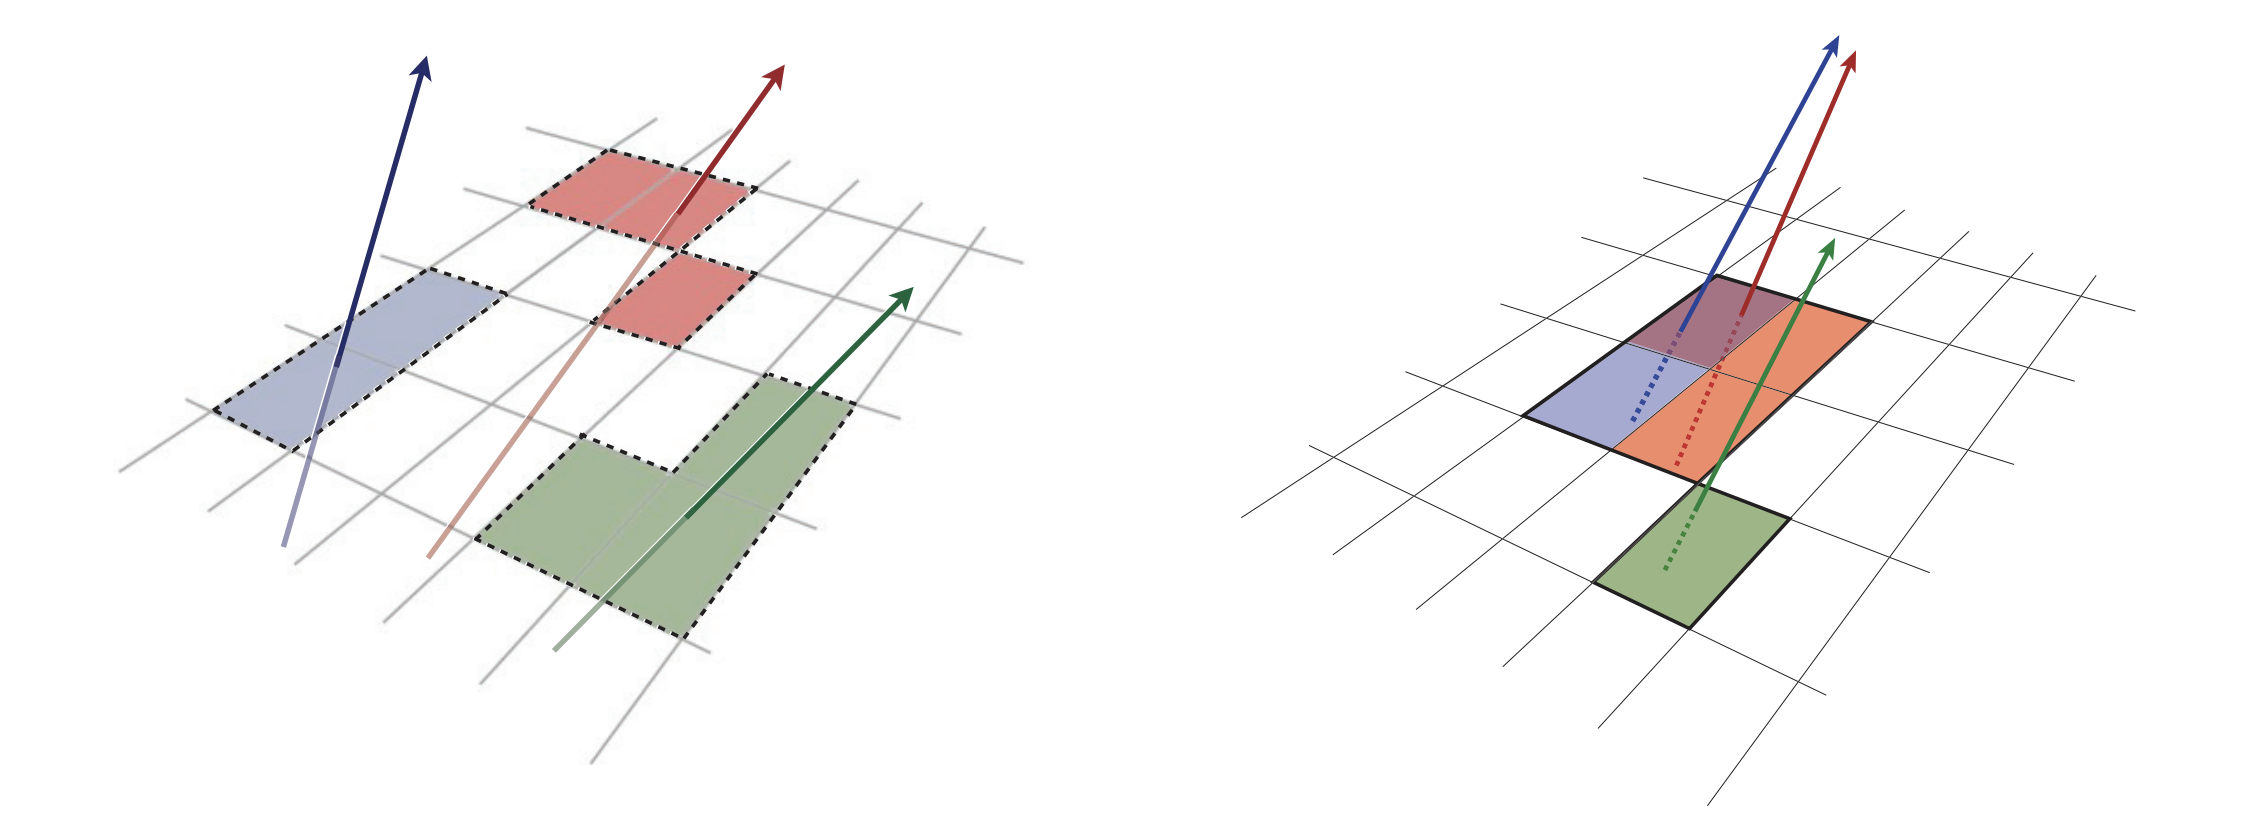
\includegraphics[width=0.8\textwidth]{chapters/2.detector/figs/merged-cluster.png}
    \caption{
      Particles (left) which have enough separation will leave charge depositions which are resolved into separate clusters.
      Sufficiently close particles (right) can lead to merged clusters.
      Their combined energy deposits are reconstructed as a single merged cluster \cite{PERF-2015-08}.}
    \label{fig:resolved/merged clusters}
\end{figure}
%

\subsubsection{Pseudotracking}\label{sec:pseudotracks}

Pseudotracking uses Monte Carlo truth information to group together all the hits left by each truth particle.
Each collection of hits which, as a unit, satisfies basic quality requirements is directly used in a full resolution track fit.
If the track fit is successful, a ``pseudotrack'' track is created and stored.
If the track fit fails, or the collection of hits does not pass the basic quality requirements (for example because of a lack of hits) then the particle is said to be un-reconstructable.
In this way, pseudotracking performance represents the ideal reconstruction performance given the ATLAS detector, with perfect hit-to-track association and and track reconstruction efficiency.
The approach was introduced in \rcite{Jansky:2013ryb} as a way to obtain a fast approximation of tracking reconstruction for simulated data, however the technique has become a useful tool for studying tracking performance in general \cite{ATL-PHYS-PUB-2015-006}.


\subsection{Vertices}\label{sec:vertex_reco}
Groups of reconstructed tracks can be examined to determine whether the particles originated from a common spatial point of origin.
This occurs when proton-proton collisions take place (primary vertices), when a particle decays or radiates, and also as a result of interaction with the detector material (secondary vertices).
Vertex reconstruction is made up of two stages.
First, vertex finding takes place, which is the process of grouping tracks into compatible vertices.
Second, vertex fitting combines information from compatible tracks to reconstruct the physical properties of the vertex, such as mass and position.

\subsubsection{Primary Vertices}
Each proton-proton interaction happens at a \textit{primary vertex} (PV).
Primary vertices are iteratively reconstructed with tracks using the iterative vertex finder (IVF) \cite{PERF-2015-01}.
%In \runthree, the IVF will be replaced with an adaptive multi-vertex finder (AMVF) \cite{ATL-PHYS-PUB-2019-015}.
The \textit{hard scatter vertex} of an event is chosen as the primary vertex whose associated tracks have the largest sum of transverse momentum squared, $\Sigma(\pt^2)$.

\subsubsection{Secondary Vertices}
Secondary vertices (SV) occur when a particle radiates or decays at a sufficient distance from the primary vertex to be resolved from the primary vertex (see \cref{sec:b_decay_topology}).
Two widely used secondary vertexing tools are used within \ATLAS: SV1 and JetFitter \cite{FTAG-2018-01,ATL-PHYS-PUB-2017-011}.
Each attempts to reconstruct secondary vertices inside a jet using the tracks associated to that jet (see \cref{sec:jet_reco} for more information about track association).
SV1 by design attempts to reconstruct only a single inclusive vertex per jet.
This inclusive vertex groups all \bhadron decay products, including tracks from the \bhadron decay itself and tracks from $b \rightarrow c$ decays.
The second tool, JetFitter attempts to resolve each displaced vertex inside the jet, such that secondary vertices from \bhadron decays are reconstructed separately to tertiary vertices from $b \rightarrow c$ decay chains.


\subsection{Jets}\label{sec:jet_reco}
Jets are an aggregate reconstructed object corresponding to a collection of collimated stable particles which results from the presence of a quark or gluon.
Jets are built by clustering constituent objects (e.g. tracks or calorimeter clusters) using a jet finding algorithm, for example the \antikt algorithm \cite{Cacciari:2008gp}, which is implemented in \textsc{FastJet}~\cite{Cacciari:2012:fastjet}.

Objects can be associated to jets in one of two ways.
The first is via a geometrical matching in $\DeltaR$ (see) 
The second is via a ghost association \cite{Cacciari:2008gn}, where the object is assigned a negligible momentum and re-clustered into the jet after its formation.

Jets from pile-up interactions are suppressed using the Jet Vertex Tagger (JVT) algorithm, which uses the transverse momenta of tracks to identify jets from pile-up interactions \cite{ATLAS-CONF-2014-018}.



\subsubsection{EMTopo Jets}
EMTopo jets are reconstructed from noise-suppressed topological clusters (topoclusters) of calorimeter energy depositions \cite{PERF-2014-07}.
The clustering uses the energy significance of each cell, defined as 
%
\begin{equation}
  S_\textnormal{cell} = \frac{E_\textnormal{cell}}{\sigma_\textnormal{noise, cell}} ,
\end{equation}
%
where $E_\textnormal{cell}$ is the energy measured in a given calorimeter cell, and $\sigma_\textnormal{noise, cell}$ is the expected level of noise on the cell (e.g. from pile-up interactions).
Topoclusters are formed from a seed cell with a large $S_\textnormal{cell}$, and expanded by iteratively adding neighbouring cells with a sufficiently large energy significance.
Collections of topoclusters are then clustered into a jet 
using the \antikt algorithm with a radius parameter of $0.4$ (\smallR jets) or $1.0$ (\largeR jets).
More information, including information on the calibration of the topocluster jet energy scale, is available in \rcite{PERF-2014-07}.


\subsubsection{Particle Flow Jets}
Particle-flow (PFlow) jets are reconstructed from particle-flow objects \cite{PERF-2015-09} using the \antikt algorithm with a radius parameter of $0.4$.
Particle-flow objects integrate information from both the ID and the calorimeters, improving the energy resolution at high transverse momenta and reducing pile-up contamination.
The PFlow jet energy scale is calibrated according to \rcite{PERF-2016-04}.

\subsubsection{\texorpdfstring{\LargeR}{Large-R} Jets}
\LargeR jets have a radius parameter $R=1.0$ and are built by clustering topological calorimeter clusters using the \antikt algorithm \cite{Butterworth:2008iy}.
The large radius parameter is especially useful for containing the decay products of a boosted Higgs boson, as discussed in \cref{chap:vhbb_boosted}. 
Due to their large size, \largeR jets benefit from a grooming procedure called trimming which remove soft contaminants inside the jet \cite{ATLAS:2020jwz,ATLAS:2013bqs}.
Trimming aims to remove jet constituents from pile-up and the underlying event, which helps to improve the jet mass resolution and its robustness to varying levels of pile-up.
The jet mass is computed using a combination of information from the calorimeters and ID, and a calibration to data is applied \cite{JETM-2018-02}.


\subsubsection{Track-jets}
Track-jets are built by clustering tracks using the \antikt clustering algorithm.
They are associated to \largeR jets as sub-jets and used to identify \largeR jets containing \bhadrons.
The radius parameter is allowed to vary with transverse momentum such that a broader cone (up to $R=0.4$) is used for \lowpt track-jets and a narrower cone (down to $R=0.02$) for \highpt track-jets \cite{Krohn:2009zg,ATL-PHYS-PUB-2017-010}.
The narrower cone is better suited to clustering highly collimated jet constituents at \highpt.

\subsubsection{Jet Flavour Labels}
Jet flavour labels are assigned to \smallR jets according to the presence of a truth hadron within ${\DeltaR(\text{hadron},\text{jet})<0.3}$ of the jet axis. If a \bhadron is found the jet is labelled a \bjet. In the absence of a \bhadron, if a \chadron is found the jet is called a \cjet.
If no \borchadrons are found, but a $\tau$ is found in the jet, it is labelled as a $\tau$-jet, else it is labelled as a \ljet.
%Jet flavour labels are assigned according to the presence of a truth hadron within ${\DeltaR(\text{hadron},\text{jet})<0.3}$ of the jet axis. If a \bhadron is found the jet is labelled a \bjet. In the absence of a \bhadron, if a \chadron is found the jet is called a \cjet.
%If no \borchadrons are found, but a $\tau$ is found in the jet, it is labelled as a $\tau$-jet, else it is labelled as a \ljet.

PFlow jets are used to train the algorithms discussed in \cref{chap:track_classification_mva} and \cref{chap:gnn_tagger}.

\subsubsection{Jet Track Association}
Tracks are associated to \smallR jets using a \DeltaR association cone, the width of which decreases as a function of jet \pt, with a maximum cone size of $\DeltaR \approx 0.45$ for jets with $\pt = \SI{20}{\GeV}$ and minimum cone size of $\DeltaR \approx 0.25$ for jets with $\pt > \SI{200}{\GeV}$. 
If a track is within the association cones of more than one jet, it is assigned to the jet which has a smaller $\DeltaR(\text{track}, \text{jet})$.


\subsection{Leptons}\label{sec:lepton_reco}

Electrons and muons leave characteristic signatures that are picked up in the ECal and MS respectively.
The reconstruction of both types of charged lepton is briefly outlined below.

\subsubsection{Electrons}

A diagrammatic view of electron reconstruction is shown in \cref{fig:electron_Reco}.
Electrons candidates are reconstructed by matching PV-compatible\footnote{The ID track associated with the electron is required to satisfy $\dzero / \dzerosig < 5$ and $\zzero\sin\theta < \SI{0.5}{\milli\meter}$.} inner detector tracks to topological calorimeter clusters.
The track-cluster matching criteria takes into account the significant energy loss of the electron due to bremsstrahlung.
If a match is found, a refit of the track is performed using the Gaussian Sum Filter (GSF) \cite{ATLAS-CONF-2012-047}, which better handles trajectory reconstruction in the presence of bremsstrahlung.
Various identification criteria are then applied to the candidates using a likelihood-based (LH) method to improve purity.
These include requirements on the track quality and cluster matching, the shape of electromagnetic shower in the ECal, leakage into the HCal, and the amount of transition radiation detected in the TRT.
Isolation criteria with respect to other nearby ID tracks and calorimeter clusters may also be applied.
A full description can be obtained from \rcite{ATLAS-CONF-2016-024}.
%
\begin{figure}[!htbp]
  \centering
  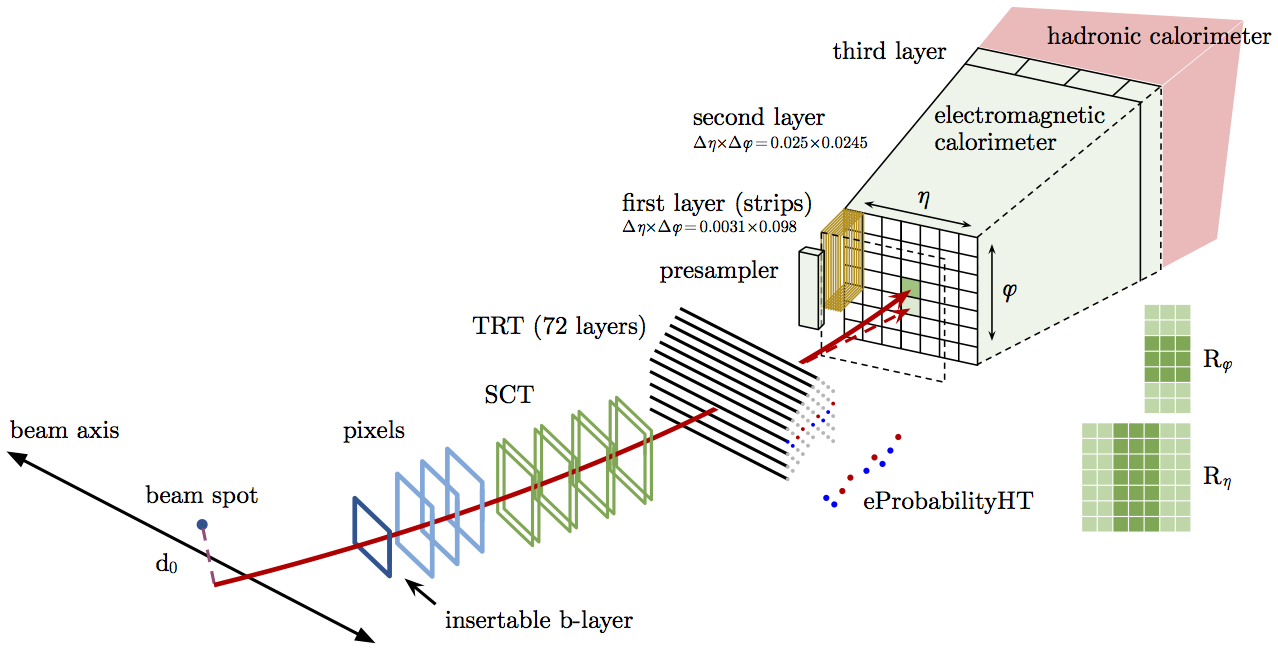
\includegraphics[width=0.8\textwidth]{chapters/2.detector/figs/electron_reco.png}
  \caption{
    A sketch of electron reconstruction using the \ATLAS detector \cite{ATLAS-CONF-2016-024}.
    Electron reconstruction makes use of the entire ID and the calorimeters.
    %In particular, discriminating information comes from the TRT and ECal.
  }
  \label{fig:electron_Reco}
\end{figure}
%


\subsubsection{Muons}
Muon reconstruction makes use of the dedicated MS (see \cref{sec:muon_spectrometer}), the tracks from the ID, and the presence of characteristic signatures in the calorimeters.
Muon tracks (i.e. a track reconstructed in the MS) are reconstructed by connecting straight-line track segments, which are identified via a Hough transform, and combined into a approximately parabolic trajectory.
Finally, a global $\chi^2$ fit is performed, taking into account possible interactions between the muon and the detector material.
A reconstructed muon is called \textit{combined} if it can be matched successfully to an to an ID track.
Combined muons undergo a further fit with the combined ID and MS hits, with the energy loss due to the traversal of the calorimeters being taking into account.

After reconstruction, candidate undergo an identification processes which helps to efficiently identify prompt muons whilst rejecting background signals (e.g. non-prompt muons from pion and kaon decays, the punch-through of a hadron from the calorimeter, or the semi-leptonic decay of a heavy flavour hadron).
Combined muon identification takes into account discrepancies in the \pt and charge measurements in the MS and ID, and the $\chi^2$ of the combined track fit.
Selections on the number of hits in the ID and MS are also applied.
At the medium identification working point, approximately \pct{96} of prompt muons with $\SI{20}{\GeV} < \pt < \SI{100}{\GeV}$ are successfully identified.
On top of the identification requirements, a number of isolation requirements can also be applied to further suppress background signals.
%In the region $|\eta| < 2.2$, the momentum resolution of reconstructed muons is \pct{1.7}.

More information on muon reconstruction, identification and isolation can be found in \rcite{PERF-2015-10}.


\subsection{Missing Transverse Momentum}\label{sec:missing_Et}

An imbalance in the final state transverse momentum can occur as a result of incomplete measurement of the final state particles.
In particular, neutrinos are not measured by the detector and contribute to the missing transverse momentum \vETmiss.
Incomplete detector acceptance and inaccuracies in the reconstruction of the final state can also contribute to the missing transverse momentum of an event.
In order to calculate the missing transverse momentum, the negative vector sum of the momentum of all photons, leptons and \smallR jets with $\pt > \SI{20}{\GeV}$ is taken.
The momenta of tracks associated to the primary vertex are also taken into account.
The magnitude of \vETmiss is written \ETmiss.
More information about missing transverse momentum reconstruction is provided in \cite{PERF-2016-07}.
